
\section{Catalan characterization}


\begin{figure}[htb]

    %\hspace{-1.5cm}
    \noindent\makebox[\textwidth]{
        \centering
        %\includegraphics[width=0.8\textwidth]{../../sympy/catalan/coloured.pdf}

        % using *angle* property to rotate it is difficult to properly align it
        % in order to have a "real" matrix representation.
        \includegraphics[width=20cm, height=20cm, keepaspectratio=true]{../sympy/catalan/catalan-traditional-standard-ignore-negatives-centered-colouring-127-rows-mod2-partitioning-triangle.pdf}
    }

    % this 'particular' line is necessary to use `displaymath' environment
    % into the caption environment, togheter with the inclusion of 
    % `caption' package. See here for more explanation:
    % http://stackoverflow.com/questions/2716227/adding-an-equation-or-formula-to-a-figure-caption-in-latex
    \captionsetup{singlelinecheck=off}
    \caption[$\mathcal{C}_{\equiv_{2}}$]{
        Modular Catalan triangle $\mathcal{C}_{\equiv_{2}}$
        \iffalse
        Catalan traditional triangle, formally: 
        \begin{displaymath}
            \mathcal{C}=\left(\frac{1-\sqrt{1-4 \, t}}{2 \, t}, \frac{1-\sqrt{1-4 \, t}}{2}\right)
        \end{displaymath} % \newline % new line no more necessary
        standard, ignore negatives, centered colouring, 127 rows, mod2 partitioning
        \fi
        }

    \label{fig:catalan-traditional-standard-ignore-negatives-centered-colouring-127-rows-mod2-partitioning-triangle}

\end{figure}

In this section we tackle a modular characterization for the Catalan array
$\mathcal{C}$ from a formal point of view. We aim at provide a proof driven
from
\autoref{fig:catalan-traditional-standard-ignore-negatives-centered-colouring-127-rows-mod2-partitioning-triangle},
and in order to accomplish this task we proceed \emph{piecewise}, breaking such
characterization into sections such that each one of them describes an
independent chunk of $\mathcal{C}$.

% inclusion of matrix expansion for C and its inverse.

\begin{table}
    \begin{displaymath} 
        \hspace{-5.5cm}
        \mathcal{C}_{10} \left(\begin{array}{rrrrrrrrrr}
        1 & 0 & 0 & 0 & 0 & 0 & 0 & 0 & 0 & 0 \\
        1 & 1 & 0 & 0 & 0 & 0 & 0 & 0 & 0 & 0 \\
        2 & 2 & 1 & 0 & 0 & 0 & 0 & 0 & 0 & 0 \\
        5 & 5 & 3 & 1 & 0 & 0 & 0 & 0 & 0 & 0 \\
        14 & 14 & 9 & 4 & 1 & 0 & 0 & 0 & 0 & 0 \\
        42 & 42 & 28 & 14 & 5 & 1 & 0 & 0 & 0 & 0 \\
        132 & 132 & 90 & 48 & 20 & 6 & 1 & 0 & 0 & 0 \\
        429 & 429 & 297 & 165 & 75 & 27 & 7 & 1 & 0 & 0 \\
        1430 & 1430 & 1001 & 572 & 275 & 110 & 35 & 8 & 1 & 0 \\
        4862 & 4862 & 3432 & 2002 & 1001 & 429 & 154 & 44 & 9 & 1
        \end{array}\right) 
        \quad
        \mathcal{C}_{10}^{-1}\left(\begin{array}{rrrrrrrrrr}
        1 & 0 & 0 & 0 & 0 & 0 & 0 & 0 & 0 & 0 \\
        1 & 0 & 0 & 0 & 0 & 0 & 0 & 0 & 0 & 0 \\
        0 & 1 & 0 & 0 & 0 & 0 & 0 & 0 & 0 & 0 \\
        0 & -1 & 1 & 0 & 0 & 0 & 0 & 0 & 0 & 0 \\
        0 & 0 & -2 & 1 & 0 & 0 & 0 & 0 & 0 & 0 \\
        0 & 0 & 1 & -3 & 1 & 0 & 0 & 0 & 0 & 0 \\
        0 & 0 & 0 & 3 & -4 & 1 & 0 & 0 & 0 & 0 \\
        0 & 0 & 0 & -1 & 6 & -5 & 1 & 0 & 0 & 0 \\
        0 & 0 & 0 & 0 & -4 & 10 & -6 & 1 & 0 & 0 \\
        0 & 0 & 0 & 0 & 1 & -10 & 15 & -7 & 1 & 0
        \end{array}\right)
    \end{displaymath}

  \caption[$\mathcal{C}$ and $\mathcal{C}^{-1}$]{Two $10$-minors of
  $\mathcal{C}$ and $\mathcal{C}^{-1}$ matrix expansions, respectively}

  \label{tab:catalan:array} 

\end{table}


\iffalse
Let $\mathcal{C}_{h}$ a principal $h$-cluster of
the Catalan array, in its traditional definition: We attempt to point out
some properties about $\mathcal{C}_{h+1}$:
\begin{itemize}
    \item a more general pattern, for any $h\in\mathcal{N}$, 
        a coefficient $d_{p^{h}-1,k}$, for $k\in\lbrace0,\ldots,p^{h}-1 \rbrace$, 
        satisfies:
        \begin{displaymath}
            d_{p^{h}-1,k} \equiv_{p} 0
        \end{displaymath}
    \item consider the subcluster $\mathcal{C}_{h}^{(0,p^{h}-1)}$ of 
        $\mathcal{C}_{h}$ obtained by removing antidiagonal $0$ (namely,
        the boundary one, composed by $1$s only) and by removing row $p^{h}-1$.
        By construction, $\mathcal{C}_{h}^{(0,p^{h}-1)}$ is a triangle too, 
        with $p^{h}-2$ coefficients per side. Therefore, $\mathcal{C}_{h+1}$
        is composed on the very top, starting at the root, by a copy of $\mathcal{C}_{h}$,
        while on the bottom there are three triangles:
        \begin{itemize}                
            \item an equilateral triangle $T_{\equiv_{p} 0}^{(h)}$, 
                with $p^{h}-1$ coefficients on each side, such that:
                \begin{displaymath}
                    d_{nk} \in T_{\equiv_{p} 0}^{(h)} \rightarrow d_{nk} \equiv_{p} 0
                \end{displaymath}
                where $n\in\lbrace p^{h},\ldots,p^{h+1}-2\rbrace$ and 
                $k\in\lbrace 0,\ldots, n-p^{h}\rbrace$, in other words
                $k\in\lbrace 0,\ldots, p^{h}(p-1)-2\rbrace$;
            \item a mirror copy of $\mathcal{C}_{h}^{(0,p^{h}-1)}$ respect column orientation,
                defining coefficients $d_{nk}$  
                where $n\in\lbrace p^{h},\ldots,p^{h+1}-2\rbrace$ and 
                $k\in\lbrace 1,\ldots, p^{h}-2\rbrace$;
            \item a segment of coefficients $d_{n, p^{h}-1} \equiv_{p} 0$ 
                where $n\in\lbrace p^{h},\ldots,p^{h+1}-2\rbrace$;
            \item a copy of $\mathcal{C}_{h}^{(0,p^{h}-1)}$,
                defining coefficients $d_{nk}$  
                where $n\in\lbrace p^{h}+1,\ldots,p^{h+1}-2\rbrace$ and 
                $k\in\lbrace p^{h},\ldots, n-1\rbrace$;
        \end{itemize}                
\end{itemize}
\fi

\subsection{Some false starts}

In order to formally proof the modular characterization of array $\mathcal{C}$, 
we begin with an attempt which applies the \emph{Lagrange Inversion Formula}. 
Write the generic element $d_{nk}\in\mathcal{C}$ using the definition:
\begin{displaymath}
    d_{nk} = [t^n] \frac{1-\sqrt{1-4\,t}}{2\,t}\,
        \left(\frac{1-\sqrt{1-4\,t}}{2}\right)^{k}
           = [t^{n+1}] \left(\frac{1-\sqrt{1-4\,t}}{2}\right)^{k+1} 
\end{displaymath}
The version of the \emph{LIF} we'll apply is the following one:
\begin{displaymath}
    \alpha\,\left[z^\alpha\right] A(z)^{\beta} = 
        \beta\,\left[w^{\alpha-\beta}\right]\Phi(w)^{\alpha}
\end{displaymath}
where $\alpha,\beta\in\mathbb{Z}$ and function $A$ relates to function
$\Phi$ according to: 
\begin{displaymath} A(z)=z\,\Phi(A(z)) \end{displaymath}
under the constraint $\Phi(0)\not=0$, otherwise a contraddiction arises
(critical relation is emphasized with $\circeq$ symbol):
\begin{displaymath} 
    z\,\Phi(0) \circeq 0 \rightarrow z\circeq\frac{0}{\Phi(0)} 
\end{displaymath}

\emph{LIF} theorem's ``from right to left'' direction allow us to make 
the following definitions:
\begin{displaymath}
    \Phi(t)=\frac{1-\sqrt{1-4\,t}}{2}\qquad \alpha=k+1\qquad \beta=k-n
\end{displaymath}
Since $\Phi(0)=0$ we cannot apply the theorem directly, so try
a combinatorial interpretation. Observe that:
\begin{displaymath}
    [t^{n+1}] \left(\frac{1-\sqrt{1-4\,t}}{2}\right)^{k+1} 
\end{displaymath}
requires to extract coefficient $n+1$ from the $(k+1)$-fold
convolution of Catalan numbers' generating function, \emph{shifted
by one place}, with itself. Before going on, be careful
to understand what coefficients are introduced; the
following expansion defines a sequence $\lbrace \hat{c}_{i}\rbrace_{i\in\mathbb{N}}$:
\begin{displaymath}
    \frac{1-\sqrt{1-4\,t}}{2} = t + t^{2} + 2 t^{3} + 5 t^{4} 
        + 14 t^{5} + 42 t^{6} + 132 t^{7} + 429 t^{8} + 1430 t^{9} 
        + \mathcal{O}\left(t^{10}\right)
\end{displaymath}
where $\hat{c}_{0}=0$. On the other hand the following one, defines a sequence 
$\lbrace c_{i}\rbrace_{i\in\mathbb{N}}$, the traditional Catalan numbers:
\begin{displaymath}
    \frac{1-\sqrt{1-4\,t}}{2\,t} = 1 + t + 2 t^{2} + 5 t^{3} + 14 t^{4} 
        + 42 t^{5} + 132 t^{6} + 429 t^{7} + 1430 t^{8} + 4862 t^{9} 
        + \mathcal{O}\left(t^{10}\right)
\end{displaymath}
so the relationship $\hat{c}_{j} = c_{j-1}$ holds for any $j\in\mathbb{N}$, 
with boundary condition $c_{-1}=0$. 

After this subtle point, there exists indices $i_{1}, i_{2}, \ldots, i_{k+1}$,
where $i_{j}\in\lbrace0,\ldots,n+1\rbrace$ for each $j\in\lbrace1,\ldots,k+1\rbrace$, 
such that:
\begin{displaymath}
    [t^{n+1}] \left(\frac{1-\sqrt{1-4\,t}}{2}\right)^{k+1} 
        = \sum_{i_{1}+ i_{2}+ \ldots+ i_{k+1}=n+1}{
            \hat{c}_{i_{1}}\,\hat{c}_{i_{2}}\,\ldots\,\hat{c}_{i_{k+1}} }
\end{displaymath}
which is the same as:
\begin{displaymath}
    [t^{n+1}] \left(\frac{1-\sqrt{1-4\,t}}{2}\right)^{k+1} 
        = \sum_{i_{1}+ i_{2}+ \ldots+ i_{k+1}=n+1}{
            c_{i_{1}-1}\,c_{i_{2}-1}\,\ldots\,c_{i_{k+1}-1} }
\end{displaymath}

Since $c_{j}$ is a Catalan coefficient, 
by definition of array $\mathcal{C}$, we observe that:
\begin{displaymath}
    c_{j} = [t^{j}]d(t)= [t^{j}]\frac{1-\sqrt{1-4\,t}}{2\,t}
\end{displaymath}
and since $\mathcal{C}$'s $A$-sequence is:
\begin{displaymath}
    A(t)=\frac{1}{1-t}
\end{displaymath}
each coefficient $c_{j}$ combines as follows:
\begin{displaymath}
    c_{j} = \sum_{k=0}^{j-1}{d_{j-1,k}}
\end{displaymath}
in other words, $c_{j}$ equals the $(j-1)$-row sum, therefore:
\marginpar{another \ac{gf} for the Catalan numbers}
\begin{displaymath}
    c_{j} = [t^{j-1}]\mathcal{C}\,A(t)
          = [t^{j-1}]d(t)\,A(h(t))
          = [t^{j}]h(t)\,A(h(t))
          = [t^{j}]\frac{1-\sqrt{1-4 \, t}}{1+\sqrt{1-4 \, t}}
\end{displaymath}
with boundary condition $c_{0}=1$, which cannot be read from the above
series expansion. Although interesting, this result is again difficult to
handle. Moreover, from the above equation, it is possible to derive
another generating function for the sequence of Catalan numbers:
\marginpar{yet another \ac{gf} for the Catalan numbers}
\begin{displaymath}
    \frac{1-\sqrt{1-4 \, t}}{1+\sqrt{1-4 \, t}}=
    \frac{\left(1-\sqrt{1-4 \, t}\right)^{2}}{4 \, t}=
    \frac{1-2\,t-\sqrt{1-4 \, t}}{2 \, t}
\end{displaymath}

Go back to identity:
\begin{displaymath}
    d_{nk} = \sum_{i_{1}+ i_{2}+ \ldots+ i_{k+1}=n+1}{
            c_{i_{1}-1}\,c_{i_{2}-1}\,\ldots\,c_{i_{k+1}-1} }
\end{displaymath}
and write a Catalan coefficient $c_{j}$ in a different form:
\begin{equation}
    c_{j} = \frac{1}{j+1}{{2j}\choose{j}} 
        = {{2j}\choose{j}} - {{2j}\choose{j+1}}
    \label{eq:catalan:coeff:rewriting}
\end{equation}
% TODO put here the reference to the bibitem.
according to article \emph{Identities induced by Riordan arrays}. This
last equation will play an important role in the following sections, in
particular when reasoning about convolutions will be hard, it will 
help in closing proofs.

\subsection{On the very first column of $\mathcal{C}_{\equiv_{2}}$}

Use \autoref{eq:catalan:coeff:rewriting}
and set a congruence relation, modulo $2$: write $j$ in base $2$, 
so there exists $k\in\mathbb{N}$ such that 
$j=j_{0} + j_{1}\,2 + j_{2}\,2^{2} + \ldots + j_{k}\,2^{k}$, where
$j_{r}\in\lbrace0,1\rbrace$, for each $r\in\lbrace0,\ldots,k\rbrace$. 
% now start distinguishing $j$ by cases: if even..., if odd...
In order to apply Lucas theorem, we proceed by cases on $j$'s parity:
\begin{itemize}
    \item let $j=2\alpha$, for some $\alpha\in\mathbb{N}$, so $j_{0}=0$,
        which make vanish the minuend:
        \begin{displaymath}
            {{2j}\choose{j+1}}
            \equiv_{2} {{0}\choose{1}}{{0}\choose{j_{1}}}{{j_{1}}\choose{j_{2}}}
                \ldots{{j_{k-1}}\choose{j_{k}}}{{j_{k}}\choose{0}}\equiv_{2}0
        \end{displaymath}
        so:
        \begin{displaymath}
            c_{j}\equiv_{2}{{2j}\choose{j}}
            \equiv_{2} {{0}\choose{0}}{{0}\choose{j_{1}}}{{j_{1}}\choose{j_{2}}}
                \ldots{{j_{k-1}}\choose{j_{k}}}{{j_{k}}\choose{0}}\equiv_{2}0
        \end{displaymath}
        \marginpar{$c_{0}$ is the only odd Catalan number among those 
            $\lbrace c_{j}\rbrace_{j\in\mathbb{N}}$ for which $j$ is even}
        A boundary case pops out when $\alpha=0$ where $j$ has to be written as 
        $j=0 + 0\cdot2 + 0\cdot2^{2} + \ldots + 0\cdot2^{k}$, therefore:
        \begin{displaymath}
            c_{0}\equiv_{2}{{0}\choose{0}}
            \equiv_{2} {{0}\choose{0}}{{0}\choose{0}}{{0}\choose{0}}
                \ldots{{0}\choose{0}}{{0}\choose{0}}\equiv_{2}1
        \end{displaymath}
        this is indeed the only case where $c_{2\alpha} \equiv_{2}1$,
        as the following alternative proof confirms:
        \begin{proof}
            Assume not, hence there exists $\hat{\alpha}\in\mathbb{N}$, greater than $0$,
            such that $c_{2\hat{\alpha}} \equiv_{2}1$. So for ${{0}\choose{j_{1}}}$
            be not zero then $j_{1}=0$; in turn, this constraint requires a new one, namely
            for ${{0}\choose{j_{2}}}$ be not zero then $j_{2}=0$; 
            in turn, this constraint requires a new one, namely
            for ${{0}\choose{j_{3}}}$ be not zero then $j_{3}=0$; 
            in turn, this constraint requires a new one, namely\ldots
            for ${{0}\choose{j_{k}}}$ be not zero then $j_{k}=0$.
            Therefore $j=0$, which contradicts the hypothesis $\alpha>0$. So,
            for even $j > 0$, coefficient $c_{j}\equiv_{2}0$, as required.
        \end{proof}

    \item let $j=2\alpha+1$, for some $\alpha\in\mathbb{N}$, so $j_{0}=1$,
        which make vanish the augend:
        \begin{displaymath}
            {{2j}\choose{j}}
            \equiv_{2} {{0}\choose{1}}{{1}\choose{j_{1}}}{{j_{1}}\choose{j_{2}}}
                \ldots{{j_{k-1}}\choose{j_{k}}}{{j_{k}}\choose{0}}\equiv_{2}0
        \end{displaymath}
        so:
        \begin{displaymath}
            c_{j}\equiv_{2}-{{2j}\choose{j+1}}
            %\equiv_{2} {{0}\choose{0}}{{0}\choose{j_{1}}}{{j_{1}}\choose{j_{2}}}
                %\ldots{{j_{k-1}}\choose{j_{k}}}{{j_{k}}\choose{0}}\equiv_{2}0
        \end{displaymath}
        observe that $(-1)^{-1}\mod2$, the multiplicative inverse of $-1$, equals $1$
        since $(-1)\cdot 1 \equiv_{2}1$, therefore we can multiply both members by
        $(-1)^{-1}\mod2$ to get:
        \begin{displaymath}
            c_{j}\equiv_{2}{{2j}\choose{j+1}}
            %\equiv_{2} {{0}\choose{0}}{{0}\choose{j_{1}}}{{j_{1}}\choose{j_{2}}}
                %\ldots{{j_{k-1}}\choose{j_{k}}}{{j_{k}}\choose{0}}\equiv_{2}0
        \end{displaymath}

        Careful handling is necessary for the term $j+1$: 
        since $j$ is odd by hypothesis, increasing it could yield a chain of carries.
        So, handling $j+1$ in a generic way, we write
        $j$ in base $2$ in its most general form, putting evidence on coefficients:
        \begin{displaymath}
            j=\left(\underbrace{1,1,\ldots,1}_{\beta},0,j_{\beta+1},\ldots,j_{\beta+\gamma}\right)_{2}
        \end{displaymath}
        where $\beta,\gamma\in\mathbb{N}$ such that $\beta>0$ and $\beta+\gamma=k$. 
        Increment by $1$:
        \begin{displaymath}
            j+1=\left(\underbrace{0,0,\ldots,0}_{\beta},1,j_{\beta+1},\ldots,j_{\beta+\gamma}%,j_{\beta+\gamma+1}
                \right)_{2}
        \end{displaymath}
        so the congruence relation gets the following shape:
        \begin{displaymath}
            c_{j}\equiv_{2}{{2j}\choose{j+1}}
                \equiv_{2} \underbrace{{{0}\choose{0}}{{1}\choose{0}}
                {{1}\choose{0}}\ldots{{1}\choose{0}}}_{\beta} 
                    {{1}\choose{1}}{{0}\choose{j_{\beta+1}}}{{j_{\beta+1}}\choose{j_{\beta+2}}}
                    \ldots{{j_{\beta+\gamma-1}}\choose{j_{\beta+\gamma}}}{{j_{\beta+\gamma}}\choose{0}}%{\beta+\gamma+1}}
        \end{displaymath}
        a simplification yield:
        \begin{displaymath}
            c_{j}\equiv_{2} {{0}\choose{j_{\beta+1}}}
                {{j_{\beta+1}}\choose{j_{\beta+2}}}
                    \ldots{{j_{\beta+\gamma-1}}\choose{j_{\beta+\gamma}}}
        \end{displaymath}
        so $c_{j}\equiv_{2} 1$ if coefficients 
            $j_{\beta+1}, \ldots, j_{\beta+\gamma-1},j_{\beta+\gamma}$
        are $0$ them all, which implies that:
        \begin{displaymath}
            j=\left(\underbrace{1,1,\ldots,1}_{\beta},\underbrace{0,0,\ldots,0}_{k-\beta+1}\right)_{2}
        \end{displaymath}

        \marginpar{$c_{2^{\alpha}-1} \equiv_{2} 1$\\Otherwise, for any $j$ odd, 
            $c_{j} \equiv_{2} 0$} 
        in other words $j = 2^{\beta+1}-1$. As boundary case, to handle $c_{1}$ correctly 
        (the above result doesn't cover it because $\beta>0$) observe:
        \begin{displaymath}
            c_{1}\equiv_{2} {{2}\choose{2}}\equiv_{2} {{0}\choose{0}}{{1}\choose{1}}\equiv_{2}1
        \end{displaymath}
\end{itemize}

In \autoref{fig:catalan-first-column} is reported a chunk of $\mathcal{C}_{\equiv_{2}}$
which shows the first column and its pattern argument of this section.
\\\\
\marginpar{using the ``classic'' closed formula on $c_{2\alpha+1}$ doesn't
    close the above proof}
It is interesting to observe that if we use the ``traditional'' characterization
of a Catalan coefficient $c_{j}$:
\begin{displaymath}
    (j+1)\,c_{j} = {{2j}\choose{j}} 
\end{displaymath}
where $j=2\alpha+1$, would've been hard to handle, because:
\begin{displaymath}
    2(\alpha+1)\,c_{j}\equiv_{2} {{0}\choose{1}}{{1}\choose{j_{1}}}
            \ldots{{j_{k-1}}\choose{j_{k}}} \equiv_{2} 0
\end{displaymath}
reduces to $0\equiv_{2}0$ identity, giving no opportunity to derive some
properties about coefficient $c_{j}$.


\begin{figure}[p]

    \noindent\makebox[\textwidth]{
        \centering
        %\includegraphics[width=0.8\textwidth]{../../sympy/catalan/coloured.pdf}

        % using *angle* property to rotate it is difficult to properly align it
        % in order to have a "real" matrix representation.
        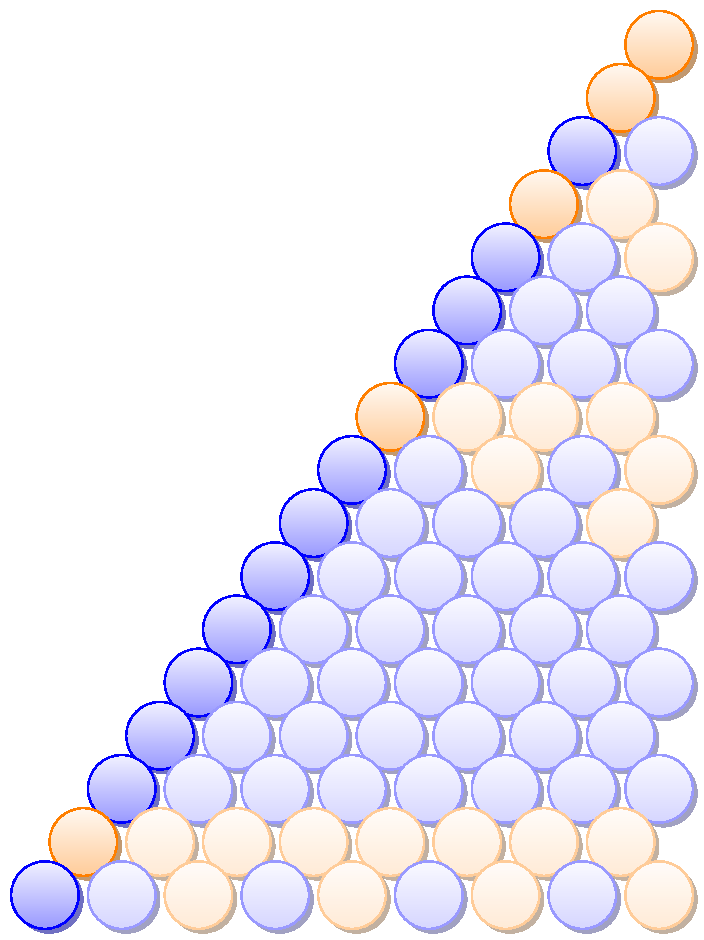
\includegraphics[
            width=7cm, 
            height=6cm, 
            keepaspectratio=true]{catalan-tikz/first-column/first-column.pdf}
    }

    % this 'particular' line is necessary to use `displaymath' environment
    % into the caption environment, togheter with the inclusion of 
    % `caption' package. See here for more explanation:
    % http://stackoverflow.com/questions/2716227/adding-an-equation-or-formula-to-a-figure-caption-in-latex
    \captionsetup{singlelinecheck=off}
    \caption[.]{ \textcolor{blue}{even},
        \textcolor{orange}{odd}  }

    \label{fig:catalan-first-column}

\end{figure}


\subsection{On rows composed of \emph{odd} coeffients only}

\begin{theorem}
    Every row $\vect{r}_{2^{\alpha}-1}$ of $\mathcal{C}_{\equiv_{2}}$, 
    for $\alpha\in\mathbb{N}$, is composed of \emph{odd} coefficients only.
\end{theorem}

\begin{proof}
    For very first coefficient $d_{2^{\alpha}-1,0}$ we have seen in the
    previous section that $d_{2^{\alpha}-1,0}\equiv_{2}1$. What about $d_{2^{\alpha}-1,1}$?
    Recall we can write it as:
    \begin{displaymath}
        d_{2^{\alpha}-1,1} = \sum_{i_{1}+ i_{2}=2^{\alpha}}{ c_{i_{1}-1}\,c_{i_{2}-1} }
    \end{displaymath}
    observe how indices $i_{1}, i_{2}$ are related: $i_{1}+ i_{2}=2^{\alpha}$,
    so $2^{\alpha}$ divides $i_{1}+i_{2}$ \emph{exactly}, so:
    \begin{displaymath}
        1 = \frac{i_{1}}{2^{\alpha}}+\frac{i_{2}}{2^{\alpha}} \qquad 
            i_{1},i_{2}\in\lbrace 0,\ldots,2^{\alpha}\rbrace
    \end{displaymath}
    %, which is the same to say that 
    %$\frac{i_{1}}{2^{\alpha}}$ and $\frac{i_{2}}{2^{\alpha}}$ are both integers.
    This implies that there exists $\beta,\gamma\in\mathbb{N}$, where $\beta,\gamma\leq\alpha$,
    such that $i_{1}=2^{\beta}$ and $i_{2}=2^{\gamma}$, respectively, since both indices
    cannot exceed $2^{\alpha}$.

    By this fact follows that $c_{i_{1}-1}=c_{2^{\beta}-1}\equiv_{2}1$ and 
    $c_{i_{2}-1}=c_{2^{\gamma}-1}\equiv_{2}1$, therefore $c_{i_{1}-1}\,c_{i_{2}-1}\equiv_{2}1$.
    By construction, fixing one index in  
    $i_{1}+ i_{2}=2^{\alpha}$ fixes the other as well: there are $2^{\alpha}+1$ available choices
    for the first index and only $1$ for the second.
    We're almost finished:
    \begin{displaymath}
        d_{2^{\alpha}-1,1} = \sum_{i_{1}+ i_{2}=2^{\alpha}}{ c_{i_{1}-1}\,c_{i_{2}-1} }
            \equiv_{2} \sum_{k=1}^{2^{\alpha}+1}{1}\equiv_{2} 2^{\alpha}+1\equiv_{2} 1
    \end{displaymath}

    What about for an arbitrary coefficient $d_{2^{\alpha}-1,s}$ where
    $s\in\lbrace{2,\ldots,2^{\alpha}-1}\rbrace$?  Recall we can write it as:
    \begin{displaymath}
        d_{2^{\alpha}-1,s} = \sum_{i_{1}+i_{2}+\ldots+i_{s+1}=2^{\alpha}}
            {c_{i_{1}-1}\,c_{i_{2}-1}\ldots\,c_{i_{s+1}-1}}
    \end{displaymath}
    Using an argument similar the previous one, from:
    \begin{displaymath}
        1 = \frac{i_{1}}{2^{\alpha}}+\ldots+\frac{i_{s+1}}{2^{\alpha}} \qquad 
            i_{j}\in\lbrace 0,\ldots,2^{\alpha}\rbrace
    \end{displaymath} 
    the generic index $i_{j}$ has to satisfy $i_{j}=2^{\alpha_{j}}$, for some
    $\alpha_{j}\leq\alpha$. Therefore $c_{i_{j}-1}\equiv_{2}1$,
    for $j\in\lbrace1,\ldots,s+1\rbrace$, and rewrite as follow:
    \begin{displaymath}
        d_{2^{\alpha}-1,s} \equiv_{2} \sum_{i_{1}+i_{2}+\ldots+i_{s+1}=2^{\alpha}}{1}
            \equiv_{2} {{s+2^{\alpha}}\choose{2^{\alpha}}}
    \end{displaymath}
    because the summation over indices $i_{1},\ldots,i_{s+1}$ asks to 
    count the number of $2^{\alpha}$-combinations of $s+1$ distinct objects,
    each of which may appear indefinitely often, that is, $0$ to $2^{\alpha}$
    times: the saught number is ${{(s+1)+2^{\alpha}-1}\choose{2^{\alpha}}}$.

    Again, we're interested on the parity of such coefficient, therefore
    write $s=s_{0}+s_{1}\,2+\ldots+s_{\alpha-1}\,2^{\alpha-1}$, because $s$ can equal 
    $2^{\alpha}-1$ at most, and apply Lucas theorem one more time:
    \begin{displaymath}
        {{s+2^{\alpha}}\choose{2^{\alpha}}}\equiv_{2} 
            {{s_{0}}\choose{0}}{{s_{1}}\choose{0}} \ldots
                {{s_{\alpha-1}}\choose{0}}{{1}\choose{1}}\equiv_{2}1 
    \end{displaymath}
    the general case holds too, therefore each coefficient lying on
    a row $\vect{r}_{2^{\alpha}-1}$ is odd, as required.
\end{proof}


\begin{figure}[p]

    \noindent\makebox[\textwidth]{
        \centering
        %\includegraphics[width=0.8\textwidth]{../../sympy/catalan/coloured.pdf}

        % using *angle* property to rotate it is difficult to properly align it
        % in order to have a "real" matrix representation.
        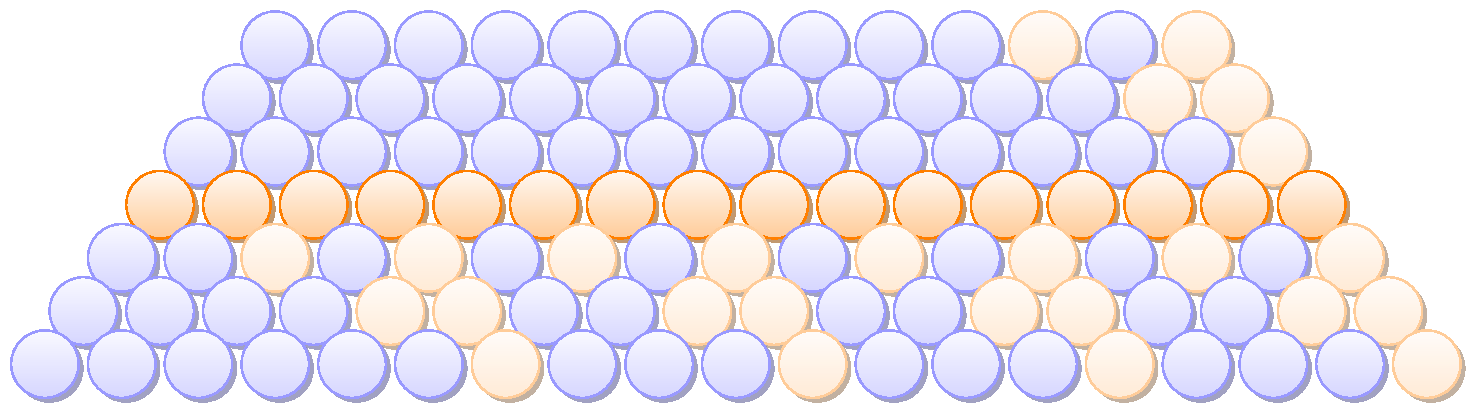
\includegraphics[width=10cm, height=10cm, keepaspectratio=true]
            {../RART2015/catalan-tikz/odd-row/odd-row.pdf}
    }

    % this 'particular' line is necessary to use `displaymath' environment
    % into the caption environment, togheter with the inclusion of 
    % `caption' package. See here for more explanation:
    % http://stackoverflow.com/questions/2716227/adding-an-equation-or-formula-to-a-figure-caption-in-latex
    \captionsetup{singlelinecheck=off}
    \caption[Row $\vect{r}_{2^{4}-1}$ of $\mathcal{C}_{\equiv_{2}}$]{
        Row $\vect{r}_{2^{4}-1}$ composed of coefficients $\textcolor{orange}{d_{2^{4}-1,s} \equiv_{2} 1}$, 
        for $s\in\lbrace1,\ldots,2^{4}-1 \rbrace$ }

    \label{fig:catalan-odd-row}

\end{figure}

In \autoref{fig:catalan-odd-row} row $\vect{r}_{2^{4}-1}$ is highlighted.

\subsection{On rows composed of alternating odd and even coefficients}

\begin{theorem}
    Let $\vect{r}_{2^{\alpha}}$ be a row of $\mathcal{C}_{\equiv_{2}}$, 
    for some $\alpha\in\mathbb{N}$. Then, exclused the very first coefficient 
        $d_{2^{\alpha},0}$ which is even, $\vect{r}_{2^{\alpha}}$ is composed of
        alternating even and odd coefficients.
\end{theorem}

\begin{proof}
    Let $d_{2^{\alpha},j}$ be a coefficient lying on row $\vect{r}_{2^{\alpha}}$,
    for some $j\in\lbrace1,\ldots,2^{\alpha}\rbrace$.

    Since $\mathcal{C}$'s $A$-sequence is:
    \begin{displaymath}
        A_{\mathcal{C}}(t)=\frac{1}{1-t}=1+t+t^{2}+t^{3}+t^{4}+t^{5}+t^{6}+t^{7}+t^{8}+
            \mathcal{O}(t^{9})
    \end{displaymath}
    it follows that $d_{2^{\alpha},j}$ can be written as the combination of $r+2$
    coefficients lying on the previous row, namely $\vect{r}_{2^{\alpha}-1}$:
    \begin{displaymath}
        d_{2^{\alpha},j} = d_{2^{\alpha}-1,j-1} +d_{2^{\alpha}-1,j} +\ldots+d_{2^{\alpha}-1,j+r} 
    \end{displaymath}
    where $r$ satisfies $r=2^{\alpha}-1-j$, so $2^{\alpha}-j+1$ coefficients are 
    combined.  By the theorem above, row $\vect{r}_{2^{\alpha}-1}$ is composed by \emph{odd}
    coefficients only, therefore proceed by cases on the parity of $j$:
    \begin{itemize}
        \item if $j$ is \emph{odd}, assume $j=2k+1$ for some $k\in\mathbb{N}$, then
            $2^{\alpha}-2k$ coefficients are combined, which is an \emph{even} number. 
            Adding an \emph{even} number of \emph{odd} numbers yield an \emph{even} number;
        \item if $j$ is \emph{even}, assume $j=2k$ for some $k\in\mathbb{N}$, then
            $2^{\alpha}-2k+1$ coefficients are combined, which is an \emph{odd} number. 
            Adding an \emph{odd} number of \emph{odd} numbers yield an \emph{odd} number.
    \end{itemize}
    therefore $d_{2^{\alpha},j}\equiv_{2}0 \leftrightarrow j=2k+1$, for 
    some $k\in\mathbb{N}$, as required.
\end{proof}


\begin{figure}[p]

    \noindent\makebox[\textwidth]{
        \centering
        %\includegraphics[width=0.8\textwidth]{../../sympy/catalan/coloured.pdf}

        % using *angle* property to rotate it is difficult to properly align it
        % in order to have a "real" matrix representation.
        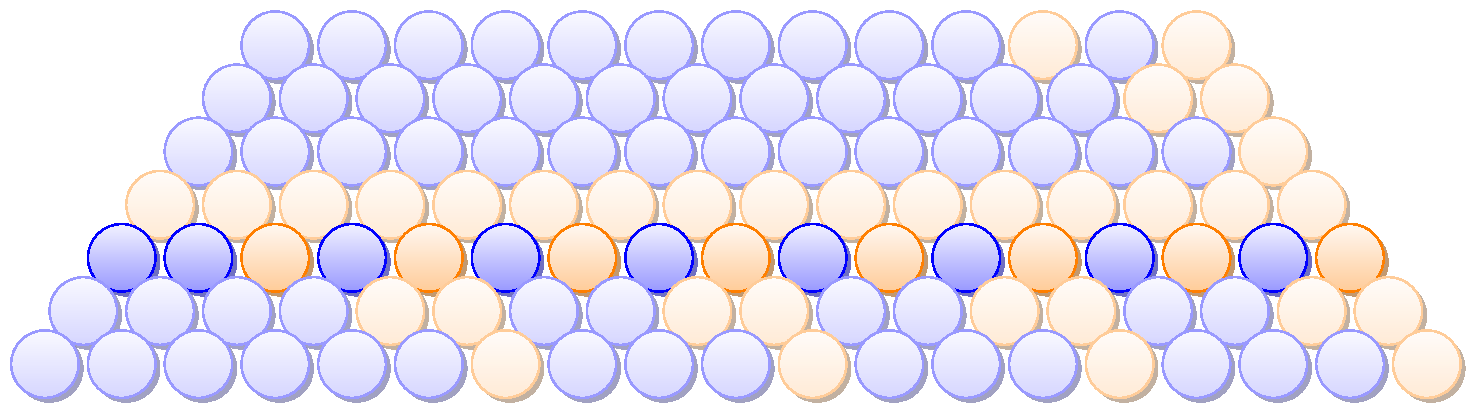
\includegraphics[width=10cm, height=3cm, keepaspectratio=true]{catalan-tikz/odd-row/alternating-row.pdf}
    }

    % this 'particular' line is necessary to use `displaymath' environment
    % into the caption environment, togheter with the inclusion of 
    % `caption' package. See here for more explanation:
    % http://stackoverflow.com/questions/2716227/adding-an-equation-or-formula-to-a-figure-caption-in-latex
    \captionsetup{singlelinecheck=off}
    \caption[.]{Row of coefficients $\textcolor{orange}{d_{2^{4}-1,s}} \equiv_{2} 1$ 
        for $s\in\lbrace1,\ldots,2^{4}-1 \rbrace$ }

    \label{fig:catalan-odd-row}

\end{figure}

In \autoref{fig:catalan-alternating-row} row $\vect{r}_{2^{4}}$ is highlighted.

\subsection{On the \flqq mirror\frqq\, segment}

\begin{theorem}
    Consider column $\vect{c}_{2^{\alpha}-1}$. 
    Each coefficient $d_{s,2^{\alpha}-1}$, for $s$ in the segment 
    $S=\lbrace2^{\alpha},\ldots,2^{\alpha+1}-2\rbrace$, is even.
\end{theorem}

\begin{proof}
As before, try to use our definition:
\begin{displaymath}
    d_{s, 2^{\alpha}-1} = \sum_{i_{1}+i_{2}+\ldots+i_{2^{\alpha}}=s+1}
        {c_{i_{1}-1}\,c_{i_{2}-1}\ldots\,c_{i_{2^{\alpha}}-1}}
\end{displaymath}
Observe that in this case, the number of Catalan coefficients
multiplied together in each summand is the same, namely $2^{\alpha}$,
for any $s\in S$; what changes respect to $s$ is the set of values 
each index $i_{j}$ can take. Look at the following table:
\begin{displaymath}
    \begin{array}{rcc}
        s = 2^{\alpha} \rightarrow
            & i_{j}\in\lbrace0,\ldots,2^{\alpha}+1\rbrace 
            & c_{k}\in\lbrace c_{-1},\ldots,c_{2^{\alpha}}\rbrace\\
        s = 2^{\alpha} +1\rightarrow
            & i_{j}\in\lbrace0,\ldots,2^{\alpha}+2\rbrace 
            & c_{k}\in\lbrace c_{-1},\ldots,c_{2^{\alpha}+1}\rbrace\\
        \vdots & & \\
        s = 2^{\alpha+1} -2\rightarrow
            & i_{j}\in\lbrace0,\ldots,2^{\alpha+1}-1\rbrace 
            & c_{k}\in\lbrace c_{-1},\ldots,c_{2^{\alpha+1}-2}\rbrace\\
    \end{array}
\end{displaymath}
therefore, for any $s\in S$, the bigger set of Catalan coefficients we have 
to consider is $\Omega = \lbrace c_{-1},\ldots,c_{2^{\alpha}-1},c_{2^{\alpha}},\ldots,c_{2^{\alpha+1}-2}\rbrace$.
Each coefficient $c_{j}\in\Omega$ is even except those of the form $c_{2^{\beta}-1}$, which are odd,
and they are $\lbrace c_{2^{\alpha-(\alpha-1)}-1},c_{2^{\alpha-(\alpha-2)}-1},\ldots, 
    c_{2^{\alpha-1}-1},c_{2^{\alpha}-1}\rbrace$, $\alpha$ in number.
Since each summand $t=c_{i_{1}-1}\,c_{i_{2}-1}\ldots\,c_{i_{2^{\alpha}}-1}$ 
has $2^{\alpha}$ coefficients, no matter if $t$ contains each coefficient in $\Omega$,
the remaining ones make it vanish and $ d_{s, 2^{\alpha}-1} \equiv_{2} 0$, for any $s\in S$,
as required.

\end{proof}


\begin{figure}[htb]

    \noindent\makebox[\textwidth]{
        \centering
        %\includegraphics[width=0.8\textwidth]{../../sympy/catalan/coloured.pdf}

        % using *angle* property to rotate it is difficult to properly align it
        % in order to have a "real" matrix representation.
        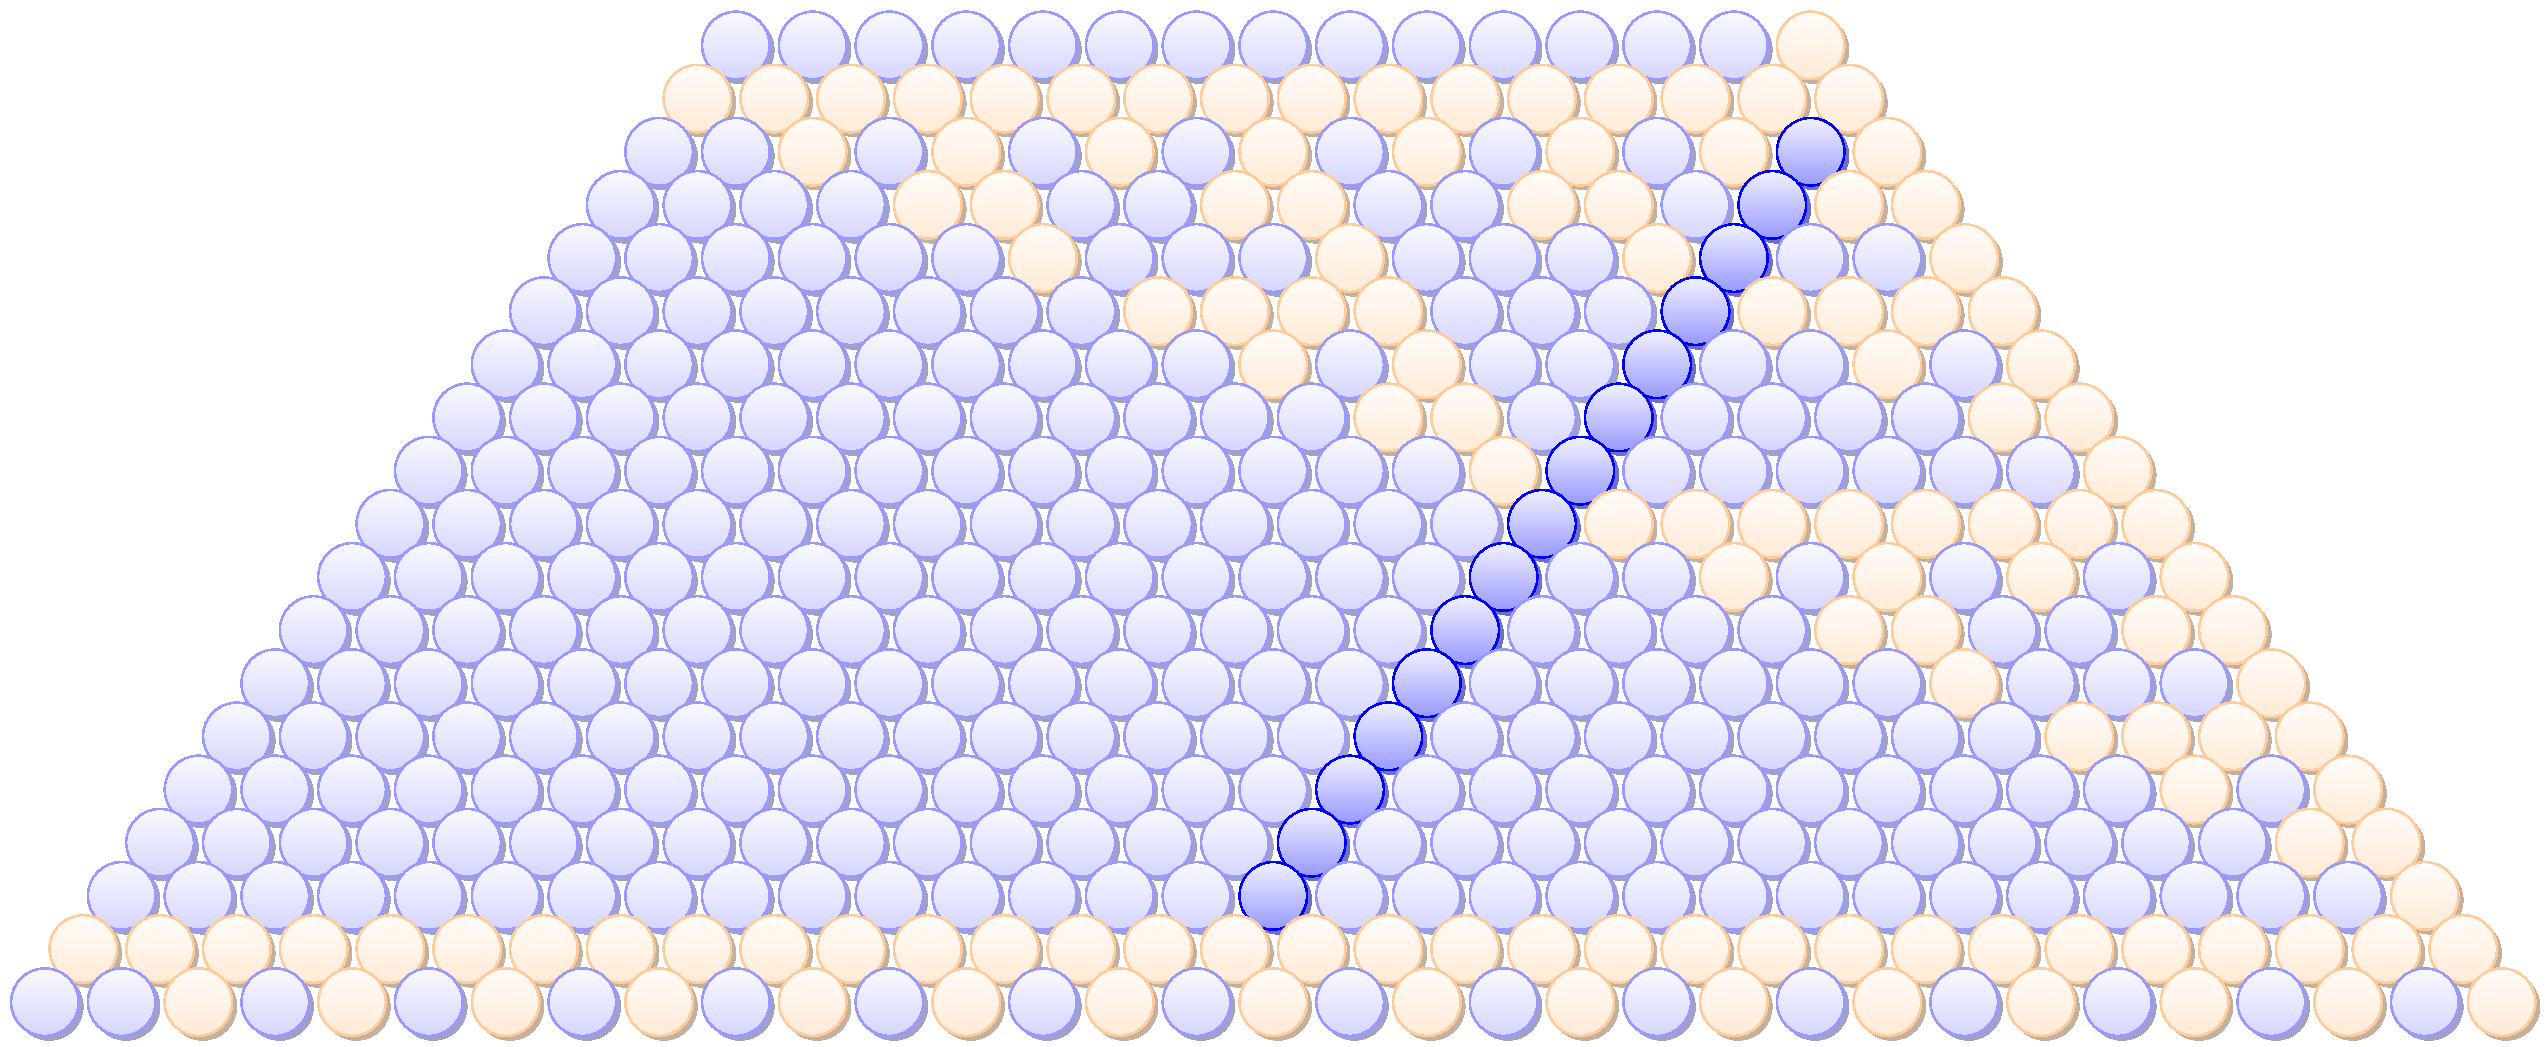
\includegraphics[width=10cm, height=10cm, keepaspectratio=true]
            {../RART2015/catalan-tikz/mirror-segment/mirror-segment.pdf}
    }

    % this 'particular' line is necessary to use `displaymath' environment
    % into the caption environment, togheter with the inclusion of 
    % `caption' package. See here for more explanation:
    % http://stackoverflow.com/questions/2716227/adding-an-equation-or-formula-to-a-figure-caption-in-latex
    \captionsetup{singlelinecheck=off}
    \caption[\emph{Mirror} segment $\Phi^{(4)}$ in $\mathcal{C}_{\equiv_{2}}^{(5)}$]
        {\emph{Mirror} segment $\Phi^{(4)}=\diagup_{\lbrace 1,2,\ldots,2^{4}-1\rbrace}^{2^{4}-1}$
        in $\mathcal{C}_{\equiv_{2}}^{(5)}$ }

    \label{fig:mirror-segment}

\end{figure}

In \autoref{fig:mirror-segment} the \flqq mirror\frqq\,segment of column $\vect{c}_{2^{4}-1}$ 
in $\mathcal{C}_{\equiv_{2}}$ is highlighted.

\subsection{On the \flqq mirrored\frqq\,segment of the \flqq mirror\frqq\, segment}


\marginpar{It should be interesting to introduce a definition for
    the mirror segment, as a pair (column c, set S), in order to avoid
    the repetition of column indices in listing coefficient in S, eventually
    they are all the same}
\begin{theorem}
    Let $\vect{c}_{2^{\alpha}-1}$ be the column on which 
    the \flqq mirror\frqq\,segment $S$ of 
    $\mathcal{C}_{\equiv_{2}}^{(\alpha+1)}$ lies. Then:
    \begin{equation}
        d_{s,s-(2^{\alpha}-1)}\equiv_{2}d_{s,2^{\alpha}-1}
    \end{equation}
    where $s\in S$.
\end{theorem}

\begin{proof}
    Use \autoref{eq:catalan:array:second:identity} on both members:
    \begin{displaymath}
        {{s+2^{\alpha}-1}\choose{2^{\alpha}-1}}- {{s+2^{\alpha}-1}\choose{2^{\alpha}-2}} \equiv_{2}
        {{2s-2^{\alpha}+1}\choose{s-2^{\alpha}+1}}- {{2s-2^{\alpha}+1}\choose{s-2^{\alpha}}}
    \end{displaymath}
    by symmetry property of binomial coefficients:
    \begin{displaymath}
        {{s+2^{\alpha}-1}\choose{s}}- {{s+2^{\alpha}-1}\choose{s+1}} \equiv_{2}
        {{2s-2^{\alpha}+1}\choose{s}}- {{2s-2^{\alpha}+1}\choose{s+1}}
    \end{displaymath}
    by simplification using $(-1)^{-1}\mod 2=1$: 
    \begin{displaymath}
        {{s+2^{\alpha}-1}\choose{s}}+ {{s+2^{\alpha}-1}\choose{s+1}} \equiv_{2}
        {{2s-2^{\alpha}+1}\choose{s}}+ {{2s-2^{\alpha}+1}\choose{s+1}}
    \end{displaymath}
    by classic recurrence rule of binomial coefficients:
    \begin{displaymath}
        {{s+2^{\alpha}}\choose{s+1}} \equiv_{2} {{2s-2^{\alpha}+2}\choose{s+1}}
    \end{displaymath}
    since $s$ can assume $2^{\alpha}$ at least and $2^{\alpha+1}-2$ at most, 
    writing $s$   in base $2$:
    \begin{displaymath}
        s=s_{0} + s_{1}2 + s_{2}2^{2}+\ldots+s_{\alpha-1}2^{\alpha-1}+2^{\alpha}
    \end{displaymath}
    and applying Lucas theorem finishes the proof:

    \begin{displaymath}
        \hspace{-2cm}
        {{s_{0}}\choose{s_{0}+1}}
        {{s_{1}}\choose{s_{1}}}
        \ldots
        {{s_{\alpha-1}}\choose{s_{\alpha-1}}}
        {{0}\choose{1}}
        {{1}\choose{0}}
        \equiv_{2}
        {{0}\choose{s_{0}+1}}
        {{s_{0}+1}\choose{s_{1}}}
        {{s_{1}}\choose{s_{2}}}
        \ldots
        {{s_{\alpha-2}}\choose{s_{\alpha-1}}}
        {{s_{\alpha-1}-1}\choose{1}}
        {{1}\choose{0}}
    \end{displaymath}
    simple algebra:
    \begin{displaymath}
        0
        \equiv_{2}
        {{0}\choose{s_{0}+1}}
        {{s_{0}+1}\choose{s_{1}}}
        {{s_{1}}\choose{s_{2}}}
        \ldots
        {{s_{\alpha-2}}\choose{s_{\alpha-1}}}
        {{s_{\alpha-1}-1}\choose{1}}
    \end{displaymath}
    \marginpar{in order to finish this proof we have to introduce a lemma about
        the row of alternating odd and even coefficient, which can be proved using
        the $A$-sequence of $\mathcal{C}$}
    By cases on the parity of $s$:
    \begin{itemize}
        \item assume $s$ is \emph{even}, therefore $s_{0}=0$ and the \ac{rhs} vanishes due to ${{0}\choose{s_{0}+1}}=0$;
        \item assume $s$ is \emph{odd}, therefore $s_{0}=1$, so apply Lucas theorem to ${{0}\choose{2}}$ again,
            yielding ${{0}\choose{2}}\equiv_{2}{{0}\choose{0}}{{0}\choose{1}}\equiv_{2}0$.
    \end{itemize}
    both cases shows that \ac{rhs} is a multiple of $p$, as required.
\end{proof}


\begin{figure}[p]

    \noindent\makebox[\textwidth]{
        \centering
        %\includegraphics[width=0.8\textwidth]{../../sympy/catalan/coloured.pdf}

        % using *angle* property to rotate it is difficult to properly align it
        % in order to have a "real" matrix representation.
        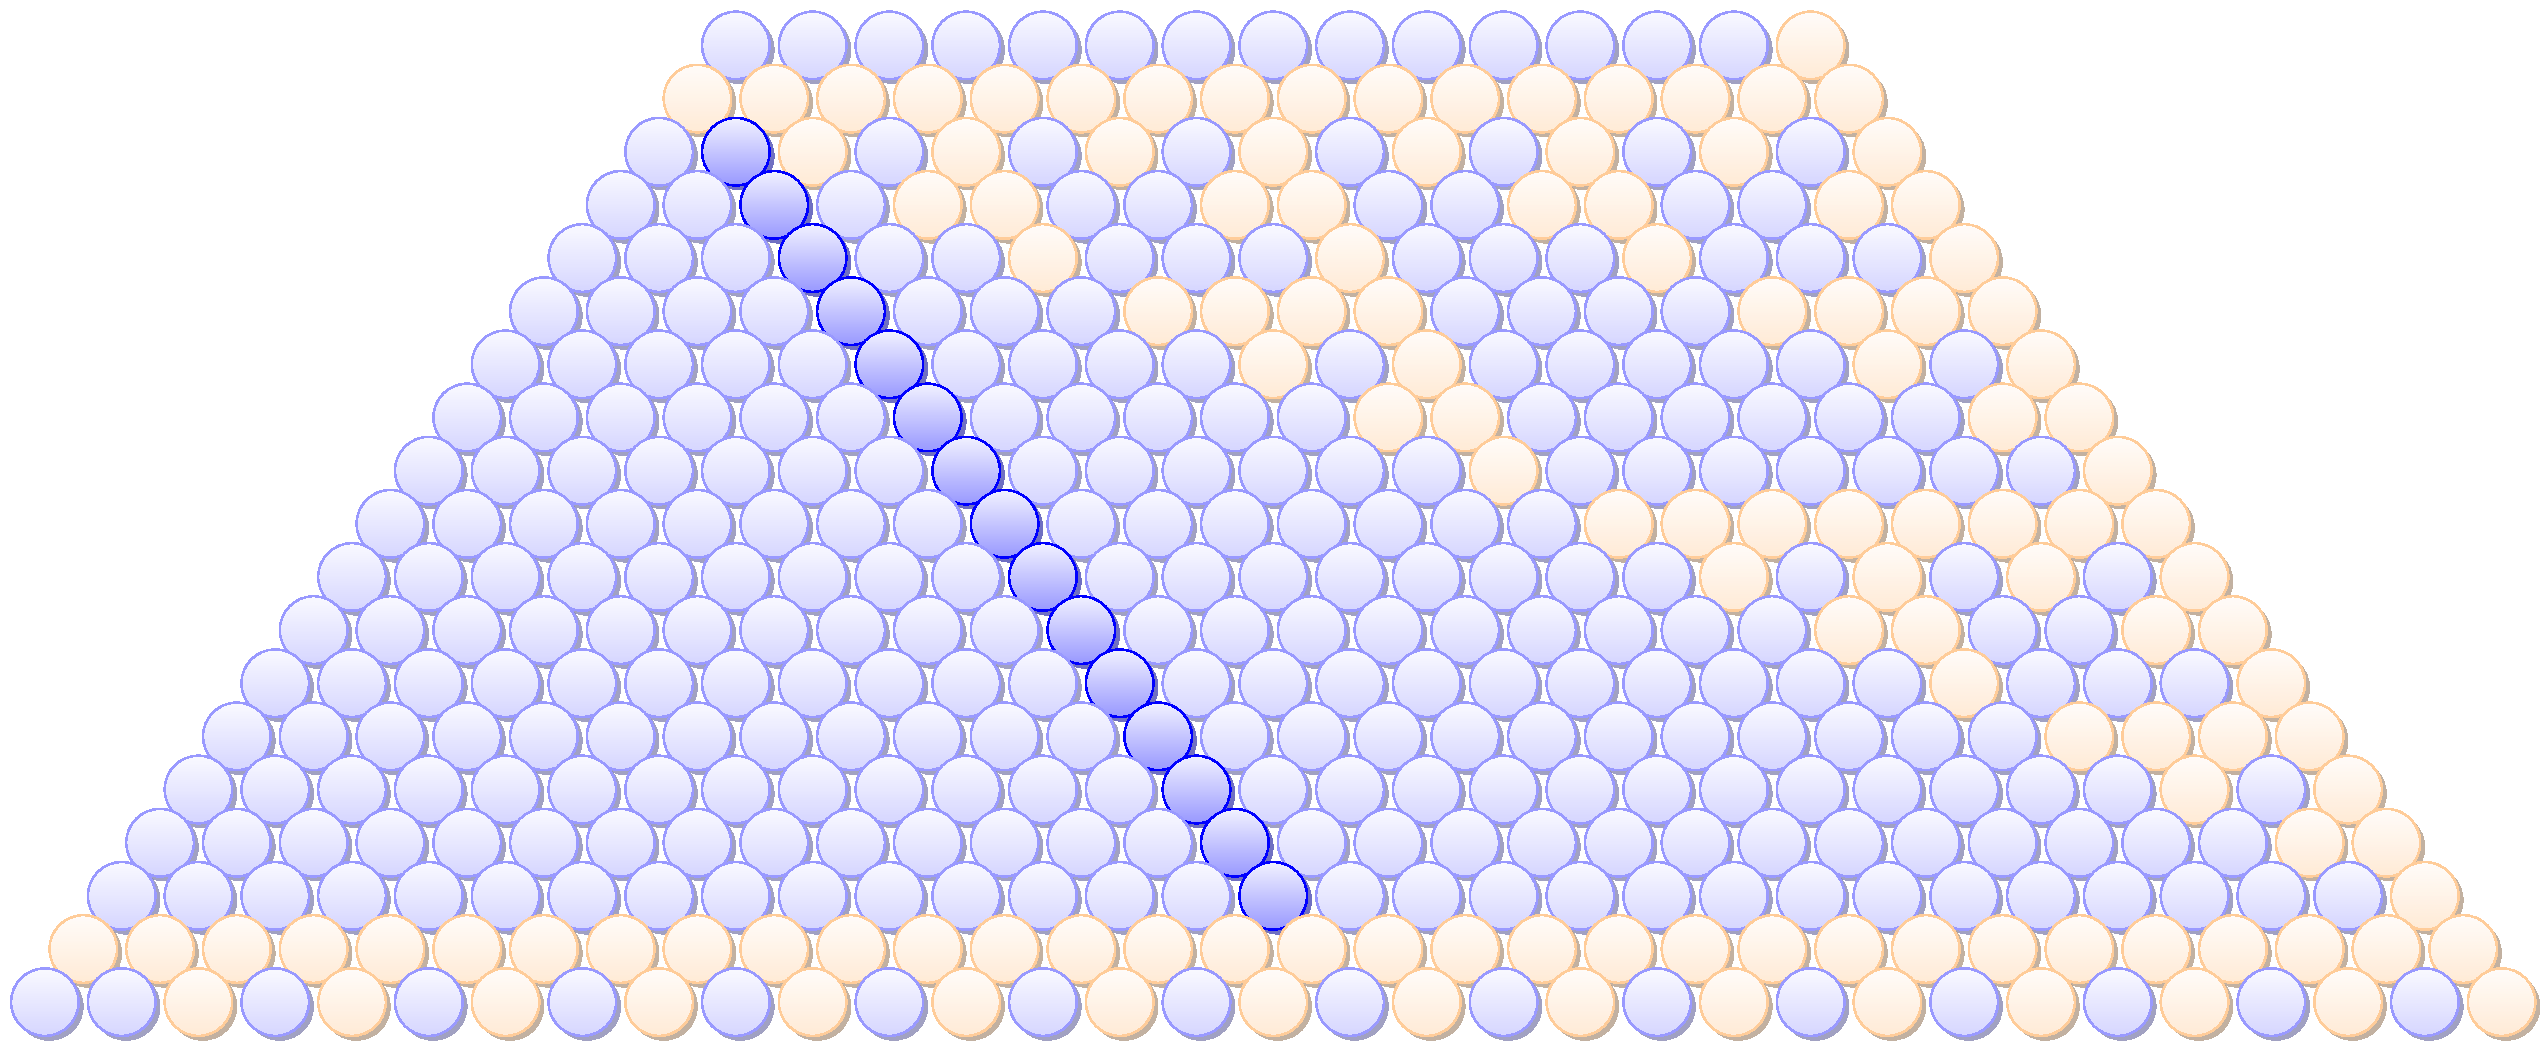
\includegraphics[width=10cm, height=10cm, keepaspectratio=true]
            {../RART2015/catalan-tikz/dual-of-mirror-segment/dual-of-mirror-segment.pdf}
    }

    % this 'particular' line is necessary to use `displaymath' environment
    % into the caption environment, togheter with the inclusion of 
    % `caption' package. See here for more explanation:
    % http://stackoverflow.com/questions/2716227/adding-an-equation-or-formula-to-a-figure-caption-in-latex
    \captionsetup{singlelinecheck=off}
    \caption[\emph{Dual} segment $\left\lbrace d_{s,s-(2^{4}-1)}\right\rbrace$,
        for $s\in rows\left(\Phi^{(4)}\right)$, in $\mathcal{C}_{\equiv_{2}}^{(5)}$]
        { \emph{Dual} segment $\left\lbrace d_{s,s-(2^{4}-1)}\right\rbrace$,
                for $s\in rows\left(\Phi^{(4)}\right)$, of \emph{mirror} segment $\Phi^{(4)}$ }



    \label{fig:dual-of-mirror-segment}

\end{figure}

In \autoref{fig:dual-of-mirror-segment} the dual of \flqq mirror\frqq\,segment in
$\mathcal{C}_{\equiv_{2}}^{(5)}$ is highlighted.

\subsection{On the \emph{upside-down} zero-hole}

Another question, this one should be interpreted keeping the
concept of principal $h$-cluster in mind:
\begin{theorem}
    Let $\mathcal{C}_{\equiv_{2}}^{(\alpha+1)}$ be a principal cluster 
    of order $\alpha+1$ of the Catalan array $\mathcal{C}$. Then, 
    $T_{\bigtriangleup}^{({\alpha})}$ denotes an \emph{upside-down} zero-hole of order $\alpha$,
    such that coefficient $d_{nk}\in T_{\bigtriangleup}^{({\alpha})}$ if 
    $n\in\lbrace 2^{{\alpha}},\ldots,2^{{\alpha}+1}-2\rbrace$ and 
    $k\in\lbrace 0,\ldots, n-2^{{\alpha}}\rbrace$. \end{theorem}

Note that $T_{\bigtriangleup}^{({\alpha})}$ is a component of the principal cluster
    of order ${\alpha}+1$.

\begin{proof}
In order to answer this question we repeatedly use the approach
of the proof about the \flqq mirror\frqq\,segment, considering the set of columns 
$\Xi=\lbrace \vect{c}_{0},\ldots, \vect{c}_{2^{{\alpha}}-2}\rbrace$ and
for each column $\vect{c}_{k}\in\Xi$, the segment of coefficients
    $S_{k}=\lbrace d_{2^{{\alpha}}+k,k},\ldots,d_{2^{{\alpha}+1}-2,k} \rbrace$.

Everything is set, so start from column on the very left, column $\vect{c}_{0}$.
So the corresponding segment $S_{0}$ is
a segment of Catalan numbers:
\begin{displaymath}
 S_{0}=\lbrace c_{2^{{\alpha}}}, \ldots, c_{2^{{\alpha}+1}-2}\rbrace
\end{displaymath}
since no coefficient $c_{j}\in S_{0}$ has the shape $c_{2^{\alpha}-1}$, 
all coefficients in $S_{0}$ are even.

Go ahead with column $\vect{c}_{1}$, so the corresponding segment is :
\begin{displaymath}
    S_{1}=\lbrace d_{2^{{\alpha}}+1,1},\ldots,d_{2^{{\alpha}+1}-2,1} \rbrace
\end{displaymath}
and coefficients in it are defined according:
\begin{displaymath}
    d_{s, 1} = \sum_{i_{1}+i_{2}=s+1} {c_{i_{1}-1}\,c_{i_{2}-1}}
\end{displaymath}
where $s\in \lbrace2^{{\alpha}}+1,\ldots,2^{{\alpha}+1}-2\rbrace$. 
This is quite similar to the proof developed for the \flqq mirror\frqq\,segment,
with the difference that summand term is composed of two coefficients, namely
$c_{i_{1}-1}\,c_{i_{2}-1}$ instead of $2^{{\alpha}}$ coefficients as in the previous proof, 
therefore the same argument applies,
since if multiplying $2^{{\alpha}}$ coefficients fails to make \emph{not} vanish
the summand term, modulo $2$, the same failure is reached if multiplying only $2$ coefficients.

The same reasoning holds for remaining columns in $\Xi$: the last one of them is 
$\vect{c}_{2^{\alpha}-2}$ (with only \emph{one} coefficient, namely $d_{2^{\alpha}-2,2^{\alpha}-2}$), 
hence $T_{\bigtriangleup}^{({\alpha})}$ is an \emph{upside-down} zero-holes of order $\alpha$,
positioned at the very left in the bottom half of $\mathcal{C}_{\equiv_{2}}^{(\alpha+1)}$, as required.

\end{proof}


\begin{figure}[p]

    \noindent\makebox[\textwidth]{
        \centering
        %\includegraphics[width=0.8\textwidth]{../../sympy/catalan/coloured.pdf}

        % using *angle* property to rotate it is difficult to properly align it
        % in order to have a "real" matrix representation.
        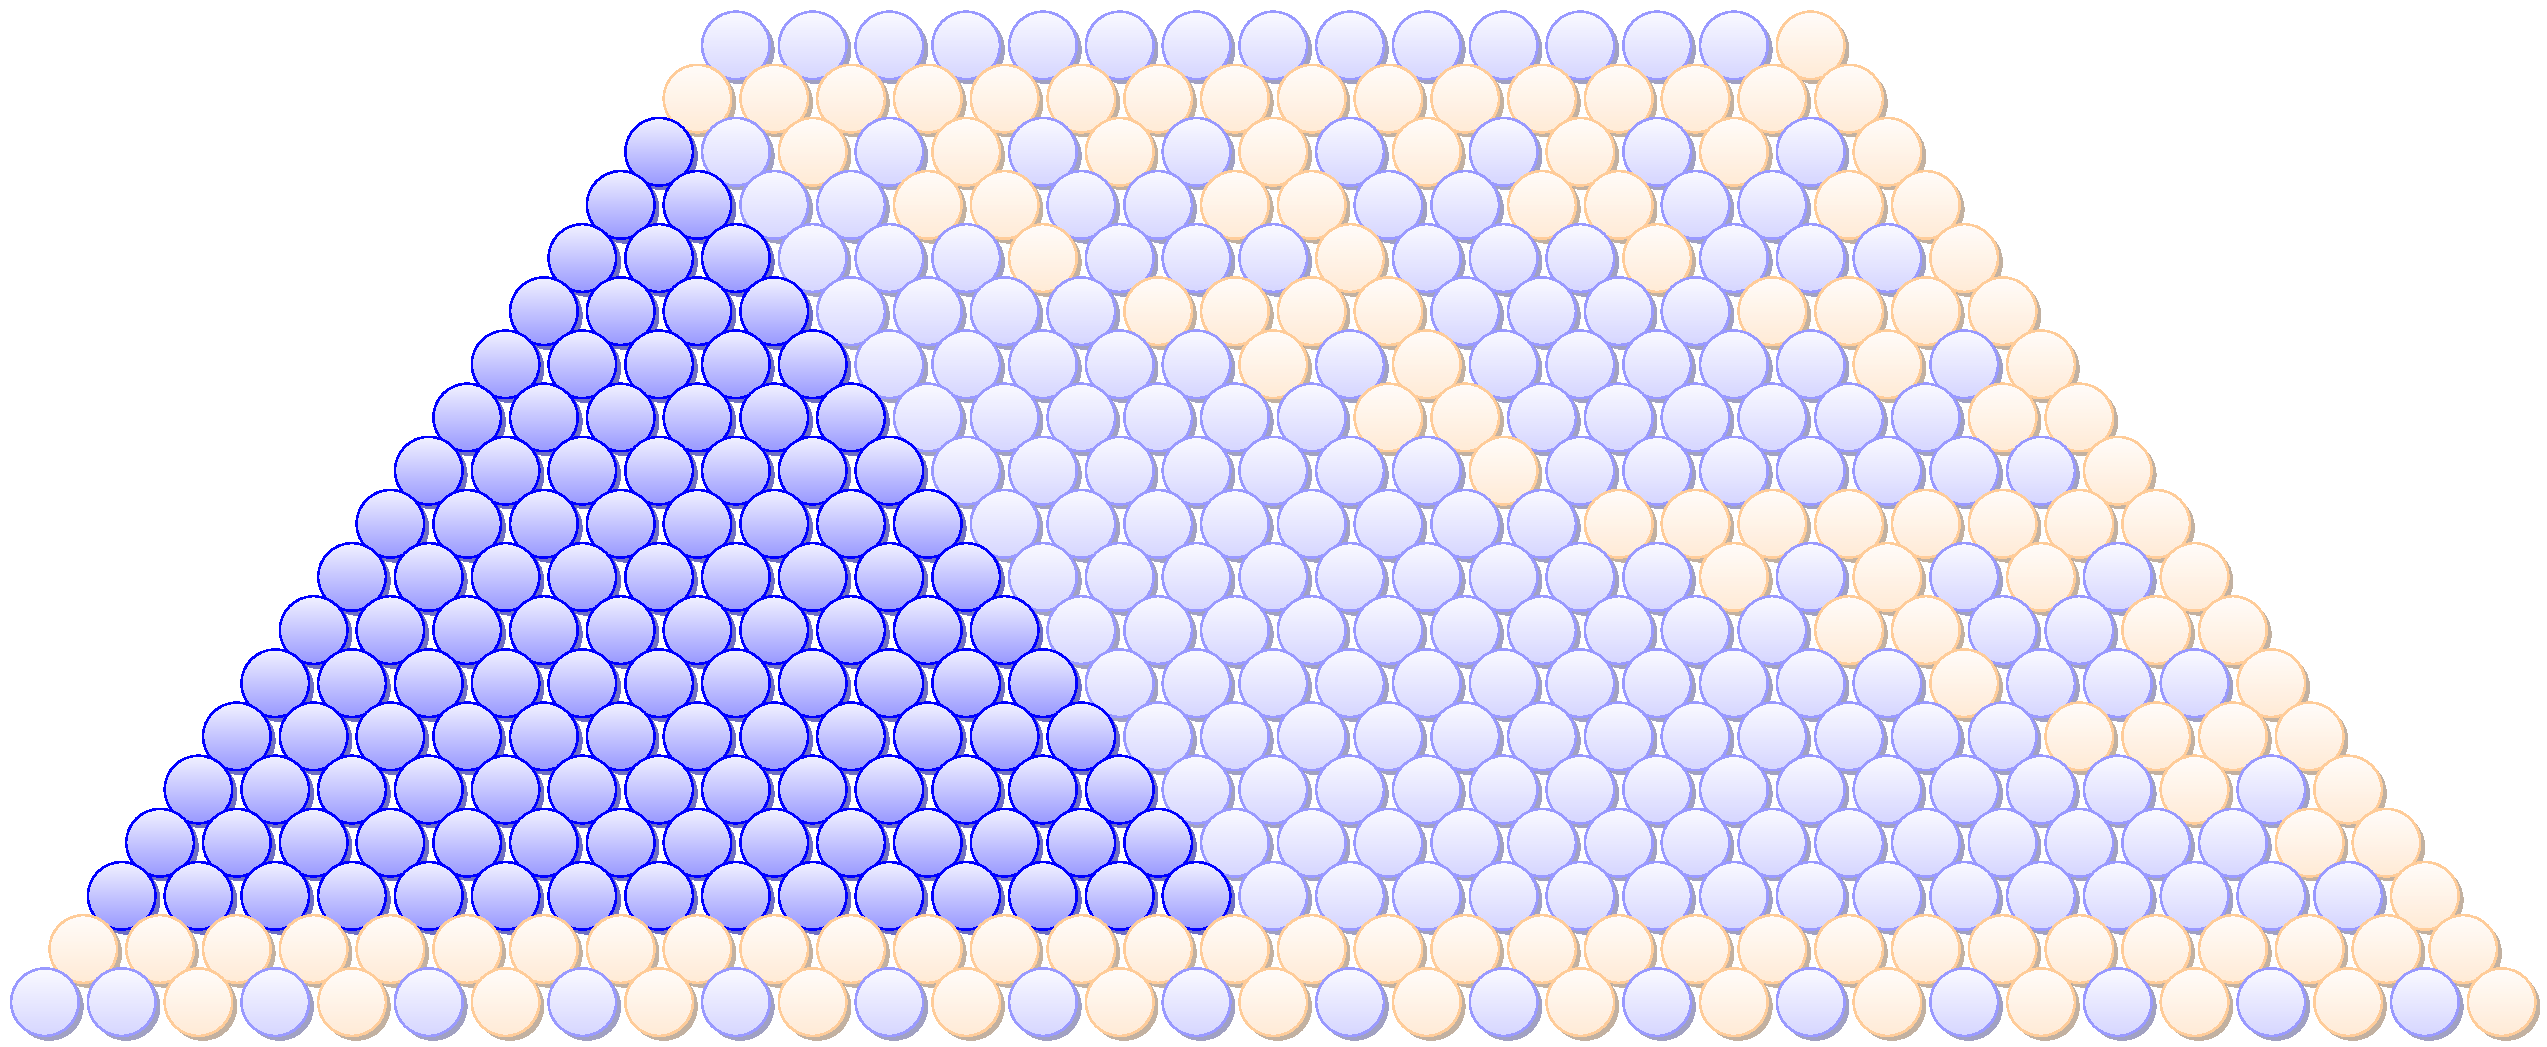
\includegraphics[width=10cm, height=10cm, keepaspectratio=true]
            {../RART2015/catalan-tikz/zero-hole/zero-hole.pdf}
    }

    % this 'particular' line is necessary to use `displaymath' environment
    % into the caption environment, togheter with the inclusion of 
    % `caption' package. See here for more explanation:
    % http://stackoverflow.com/questions/2716227/adding-an-equation-or-formula-to-a-figure-caption-in-latex
    \captionsetup{singlelinecheck=off}
    \caption[Upside-down zero-hole $T_{\bigtriangleup}^{(4)}$ within
        $\mathcal{C}_{\equiv_{2}}^{(\alpha+1)}$]{Zero hole $T_{\bigtriangleup}^{(4)} \subset \mathcal{C}_{\equiv_{2}}^{(5)}$}

    \label{fig:catalan-zero-hole}

\end{figure}

In \autoref{fig:catalan-zero-hole} is reported $T_{\bigtriangleup}^{(4)}$.

\subsection{On two \flqq mirrored\frqq\,clusters}

\begin{theorem}
    Consider column $\vect{c}_{2^{{\alpha}}-1}$, as the one considered 
    for the introduction of the \flqq mirror\frqq\,segment, and let 
    $\hat{d}_{s,2^{{\alpha}}-1}$ be a coefficient, such that $s$ is in the segment 
    $S=\lbrace2^{\alpha}+1,\ldots,2^{\alpha+1}-2\rbrace$. Then:
    \begin{displaymath}
        d_{s-e,2^{{\alpha}}-1-e} \equiv_{2} d_{s,2^{{\alpha}}-1+e}
    \end{displaymath}
    for $e\in\lbrace1,\ldots,s-(2^{{\alpha}}-1)-1\rbrace=\lbrace1,\ldots,s-2^{{\alpha}}\rbrace$,
    computed looking at row $s$ toward its end.
\end{theorem}

Using our definition we can rewrite as:

\begin{lenghtydisplaymath}
    \sum_{i_{1}+i_{2}+\ldots+i_{2^{\alpha}-e}=s-e+1}
        {c_{i_{1}-1}\,c_{i_{2}-1}\ldots\,c_{i_{2^{\alpha}-e}-1}}
    \equiv_{2}
    \sum_{i_{1}+i_{2}+\ldots+i_{2^{\alpha}+e}=s+1}
        {c_{i_{1}-1}\,c_{i_{2}-1}\ldots\,c_{i_{2^{\alpha}+e}-1}}
\end{lenghtydisplaymath}

Panic! No idea to tackle the general setting as a whole. So, start small.
Let $s=2^{{\alpha}}+1$, therefore no choices for $e$, obliged $e=1$, so:

\begin{lenghtydisplaymath}
    \sum_{i_{1}+i_{2}+\ldots+i_{2^{\alpha}-1}=2^{{\alpha}}+1}
        {c_{i_{1}-1}\,c_{i_{2}-1}\ldots\,c_{i_{2^{\alpha}-1}-1}}
    \equiv_{2}
    \sum_{i_{1}+i_{2}+\ldots+i_{2^{\alpha}+1}=2^{{\alpha}}+2}
        {c_{i_{1}-1}\,c_{i_{2}-1}\ldots\,c_{i_{2^{\alpha}+1}-1}}
\end{lenghtydisplaymath}

too difficult to proceed this way, too. 

\iffalse
Another idea could be to
translate back columns (discarding unnecessary coefficients by subtracting them)
on the \emph{left} of the choosen ``pivot'' element $\hat{d}_{s,2^{{\alpha}}-1}$. 
In this way columns should be congruent element-wise but, again, it seems difficult
to move forward this way.
\fi

Another approach is to find a closed form for a coefficient in $\mathcal{C}$,
using the extract operator: $d_{nk} = [t^{n}]d_{\mathcal{C}}(t)h_{\mathcal{C}}(t)^{k}$.
According the article \emph{Identities induced by Riordan Arrays}, such
coefficient $d_{nk}$ agrees with the following identities:
\begin{equation}
    d_{nk}=\frac{k+1}{n+1}{{2n-k}\choose{n-k}}
    \label{eq:catalan:array:first:identity}
\end{equation}
    \marginpar{in these ``modular''
        proofs it's much easier to rewrite a binomial coefficient
        into other binomial coefficients, only}
or else:
\begin{equation}
    d_{nk}={{2n-k}\choose{n-k}} - {{2n-k}\choose{n-k-1}}
    \label{eq:catalan:array:second:identity}
\end{equation}

We attempt a \emph{false start} using the first one.
\begin{proof}
Assume not, therefore we need to yield a contraddiction if:
\begin{displaymath}
    d_{s-e,2^{{\alpha}}-1-e} \not\equiv_{2} d_{s,2^{{\alpha}}-1+e}
\end{displaymath}
holds. Rewriting the congruence according \autoref{eq:catalan:array:first:identity}
 for $d_{nk}$:
\begin{displaymath}
    \frac{2^{{\alpha}}-e}{s-e+1}{{2(s-e)-(2^{{\alpha}}-1-e)}\choose{s-e-(2^{{\alpha}}-1-e)}}
    \not\equiv_{2}
    \frac{2^{{\alpha}}+e}{s+1}{{2s-(2^{{\alpha}}-1+e)}\choose{s-(2^{{\alpha}}-1+e)}}
\end{displaymath}
simplify it:
\begin{displaymath}
    \frac{2^{{\alpha}}-e}{s-e+1}{{2s-e-2^{{\alpha}}+1}\choose{s-2^{{\alpha}}+1}}
    \not\equiv_{2}
    \frac{2^{{\alpha}}+e}{s+1}{{2s-2^{{\alpha}}+1-e}\choose{s-2^{{\alpha}}+1-e}}
\end{displaymath}
manipulate using ${{n}\choose{k}}={{n}\choose{n-k}}$:
\begin{displaymath}
    \frac{2^{{\alpha}}-e}{s-e+1}{{2s-e-2^{{\alpha}}+1}\choose{s-e}}
    \not\equiv_{2}
    \frac{2^{{\alpha}}+e}{s+1}{{2s-2^{{\alpha}}+1-e}\choose{s}}
\end{displaymath}
dead end: nonetheless binomial coeffients allow some grunging,
fractions on both side are difficult to handle since it's hard
to find their multiplicative inverses, modulo $2$.
\end{proof} 

Trace back to \autoref{eq:catalan:array:second:identity} for coefficient $d_{nk}$. 
\begin{proof}
Recall we would like to prove the following statement:
\begin{displaymath}
    d_{s-e,2^{{\alpha}}-1-e} \equiv_{2} d_{s,2^{{\alpha}}-1+e}
\end{displaymath}
Rewrite the left hand side:
\begin{displaymath}
    d_{s-e,2^{{\alpha}}-1-e}= {{2(s-e)-(2^{{\alpha}}-1-e)}\choose{(s-e)-(2^{{\alpha}}-1-e)}}
        - {{2(s-e)-(2^{{\alpha}}-1-e)}\choose{(s-e)-(2^{{\alpha}}-1-e)-1}}
\end{displaymath}
in the same spirit, rewrite the right hand side:
\begin{displaymath}
    d_{s,2^{{\alpha}}-1+e}={{2s-(2^{{\alpha}}-1+e)}\choose{s-(2^{{\alpha}}-1+e)}}
        - {{2s-(2^{{\alpha}}-1+e)}\choose{s-(2^{{\alpha}}-1+e)-1}}
\end{displaymath}
therefore:
\begin{displaymath}
    \begin{split}
        {{2s-e-2^{{\alpha}}+1}\choose{s-2^{{\alpha}}+1}}
            - {{2s-e-2^{{\alpha}}+1}\choose{s-2^{{\alpha}}}}
        &\equiv_{2}
        {{2s-2^{{\alpha}}+1-e}\choose{s-2^{{\alpha}}+1-e}}
            - {{2s-2^{{\alpha}}+1-e}\choose{s-2^{{\alpha}}-e}}\\
        {{2s-e-2^{{\alpha}}+1}\choose{s-e}}
            - {{2s-e-2^{{\alpha}}+1}\choose{s-e+1}}
        &\equiv_{2}
        {{2s-2^{{\alpha}}+1-e}\choose{s}}
            - {{2s-2^{{\alpha}}+1-e}\choose{s+1}}\\
    \end{split}
\end{displaymath}

Since $e\in\lbrace1,\ldots,s-2^{{\alpha}}\rbrace$, proceed by complete induction on $e$:
\begin{itemize}
    \item base case $e=1$ yield the following congruence:
        \begin{displaymath}
                {{2s-2^{{\alpha}}}\choose{s-1}}-{{2s-2^{{\alpha}}}\choose{s}}
                \equiv_{2}
                {{2s-2^{{\alpha}}}\choose{s}}-{{2s-2^{{\alpha}}}\choose{s+1}}\\
        \end{displaymath}
        which is the same to say:
        \begin{displaymath}
                {{2s-2^{{\alpha}}}\choose{s-1}}+{{2s-2^{{\alpha}}}\choose{s+1}} \equiv_{2} 0
        \end{displaymath}
        let $s=s_{0}+s_{1}\,2+s_{2}\,2^{2}+\ldots+s_{{\alpha}-1}\,2^{{\alpha}-1} + 2^{{\alpha}}$
        be the generic representation of $s$ in base $2$, since 
        $s\in\lbrace 2^{{\alpha}}+1,\ldots,2^{{\alpha}+1}-2 \rbrace$; also  
        let $2s-2^{{\alpha}}=s_{0}\,2+s_{1}\,2^{2}+s_{2}\,2^{3}+\ldots+s_{{\alpha}-1}^{*}\,2^{{\alpha}} + s_{{\alpha}}^{*}\,2^{{\alpha}+1}$,
        where $(s_{{\alpha}-1}^{*},s_{{\alpha}}^{*})$ equals $(0,1)$ if $s_{{\alpha}-1}=1$, otherwise equals $(1,0)$.
        By cases on the parity of $s$:
        \begin{itemize}
            \item assume $s$ even, therefore both $s-1$ both $s+1$ are odd, 
                let $\hat{s}=1+\hat{s}_{1}\,2+\hat{s}_{2}\,2^{2}+\ldots+
                    \hat{s}_{{\alpha}-1}\,2^{{\alpha}-1}+2^{{\alpha}}$ be one of them, hence:
                \begin{displaymath}
                        {{2s-2^{{\alpha}}}\choose{\hat{s}}}  
                        \equiv_{2}
                        {{0}\choose{1}} 
                        {{0}\choose{\hat{s}_{1}}}
                        {{s_{1}}\choose{\hat{s}_{2}}}
                        \ldots
                        {{s_{{\alpha}-2}}\choose{\hat{s}_{{\alpha}-1}}}
                        {{s_{{\alpha}-1}^{*}}\choose{1}}
                        {{s_{{\alpha}}^{*}}\choose{0}} = 0
                \end{displaymath}
                Observe $\hat{s}_{{\alpha}}=1$ against boundary cases:
                if $s=2^{{\alpha}}+1$ then $\hat{s}=s-1=2^{{\alpha}}$, on the other
                hand if $s=2^{{\alpha}+1}-2$ then $\hat{s}=s+1=2^{{\alpha}+1}-1$,
                therefore in both cases the coefficient of $2^{{\alpha}}$ is $1$.
                Eventually we get $0+0 \equiv_{2}0$, which holds;

            \item assume $s$ odd, therefore both $s-1$ both $s+1$ are even, 
                let's study the former:
                \begin{displaymath}
                        {{2s-2^{{\alpha}}}\choose{s-1}}  
                        \equiv_{2}
                        {{0}\choose{0}} 
                        {{1}\choose{s_{1}}}
                        {{s_{1}}\choose{s_{2}}}
                        \ldots
                        {{s_{{\alpha}-2}}\choose{s_{{\alpha}-1}}}
                        {{s_{{\alpha}-1}^{*}}\choose{1}}
                        {{s_{{\alpha}}^{*}}\choose{0}}
                \end{displaymath}
                in order for the right hand side to not vanish, modulo $2$,
                it is mandatory for coefficients $\lbrace s_{i}\rbrace_{i\in\lbrace1,\ldots,{\alpha}-2\rbrace}$
                to satisfy $s_{i}\geq s_{i+1}$: if any one of them is $0$, say $s_{j}$, then
                $s_{j+1},\ldots,s_{j+k}$, with $j+k={\alpha}-1$,
                have to be all $0$ too. In particular, if $s_{{\alpha}-1}=0$ then 
                $(s_{{\alpha}-1}^{*},s_{{\alpha}}^{*})=(1,0)$
                therefore the right hand side reduces to $1$, modulo $2$.
                Observe that coefficients $\lbrace s_{i}\rbrace_{i\in\lbrace1,\ldots,{\alpha}-2\rbrace}$
                cannot be all $1$ otherwise 
                $s=(\underbrace{1,1,1,\ldots,1}_{{\alpha}+1})_{2}=2^{{\alpha}+1}-1$ raises a contraddiction, because
                $s$ can assume $2^{{\alpha}+1}-2$ at most. 
                
                For the latter, namely $s+1$, assume $s$ can be represented as 
                $(\underbrace{1,1,\ldots,1}_{r},0,s_{r+1},s_{r+2},\ldots,s_{{\alpha}-1},1)_{2}$, for
                $r\in\lbrace1,\ldots,{\alpha}-2\rbrace$, since a $0$ must occur otherwise $s=2^{{\alpha}+1}-1$
                which cannot be the case, as we've already seen.  Adding $1$ yield the representation
                $(\underbrace{0,0,\ldots,0}_{r},1,s_{r+1},s_{r+2},\ldots,s_{{\alpha}-1},1)_{2}$, therefore:
                \begin{lenghtydisplaymath}
                        {{2s-2^{{\alpha}}}\choose{s+1}} 
                        \equiv_{2} 
                        \underbrace{
                            {{0}\choose{0}} 
                            {{1}\choose{0}}
                            {{1}\choose{0}}
                            \ldots
                            {{1}\choose{0}}
                        }_{r}
                        {{1}\choose{1}}
                        {{0}\choose{s_{r+1}}}
                        {{s_{r+1}}\choose{s_{r+2}}}
                        \ldots
                        {{s_{{\alpha}-2}}\choose{s_{{\alpha}-1}}}
                        {{s_{{\alpha}-1}^{*}}\choose{1}}
                        {{s_{{\alpha}}^{*}}\choose{0}}
                \end{lenghtydisplaymath}
                In order to not vanish, modulo $2$, 
                $s_{r+1}=0$, this propagates in turn that $s_{r+2}=0$, \ldots, 
                this propagates in turn that $s_{{\alpha}-2}=0$,
                this propagates in turn that $s_{{\alpha}-1}=0$. But if $s_{{\alpha}-1}=0$
                then $(s_{{\alpha}-1}^{*},s_{{\alpha}}^{*})=(1,0)$, therefore the right
                hand side reduces to $1$.

                Combining the above cases for $s$ odd we reach:
                \begin{displaymath}
                        {{2s-2^{{\alpha}}}\choose{s-1}}+{{2s-2^{{\alpha}}}\choose{s+1}} \equiv_{2} 1+1\equiv_{2} 0
                \end{displaymath}
        \end{itemize}

        \item assume the argument holds for $k\leq e$ and prove for $k=e+1$, so we need to show:

            \begin{lenghtydisplaymath}
                \begin{split}
                    {{2s-(e+1)-2^{{\alpha}}+1}\choose{s-2^{{\alpha}}+1}}
                        - {{2s-(e+1)-2^{{\alpha}}+1}\choose{s-2^{{\alpha}}}}
                    &\equiv_{2}
                    {{2s-2^{{\alpha}}+1-(e+1)}\choose{s-2^{{\alpha}}+1-(e+1)}}
                        - {{2s-2^{{\alpha}}+1-(e+1)}\choose{s-2^{{\alpha}}-(e+1)}}\\
                    {{2s-(e+1)-2^{{\alpha}}+1}\choose{s-(e+1)}}
                        - {{2s-(e+1)-2^{{\alpha}}+1}\choose{s-(e+1)+1}}
                    &\not\equiv_{2}
                    {{2s-2^{{\alpha}}+1-(e+1)}\choose{s}}
                        - {{2s-2^{{\alpha}}+1-(e+1)}\choose{s+1}}\\
                    {{2s-e-2^{{\alpha}}}\choose{s-e-1}}
                        - {{2s-e-2^{{\alpha}}}\choose{s-e}}
                    &\not\equiv_{2}
                    {{2s-2^{{\alpha}}-e}\choose{s}}
                        - {{2s-2^{{\alpha}}-e}\choose{s+1}}\\
                \end{split}
            \end{lenghtydisplaymath}
            which follows directly by complete induction hypothesis.
\end{itemize}

\end{proof}


\begin{figure}[htb]

    \noindent\makebox[\textwidth]{
        \centering
        %\includegraphics[width=0.8\textwidth]{../../sympy/catalan/coloured.pdf}

        % using *angle* property to rotate it is difficult to properly align it
        % in order to have a "real" matrix representation.
        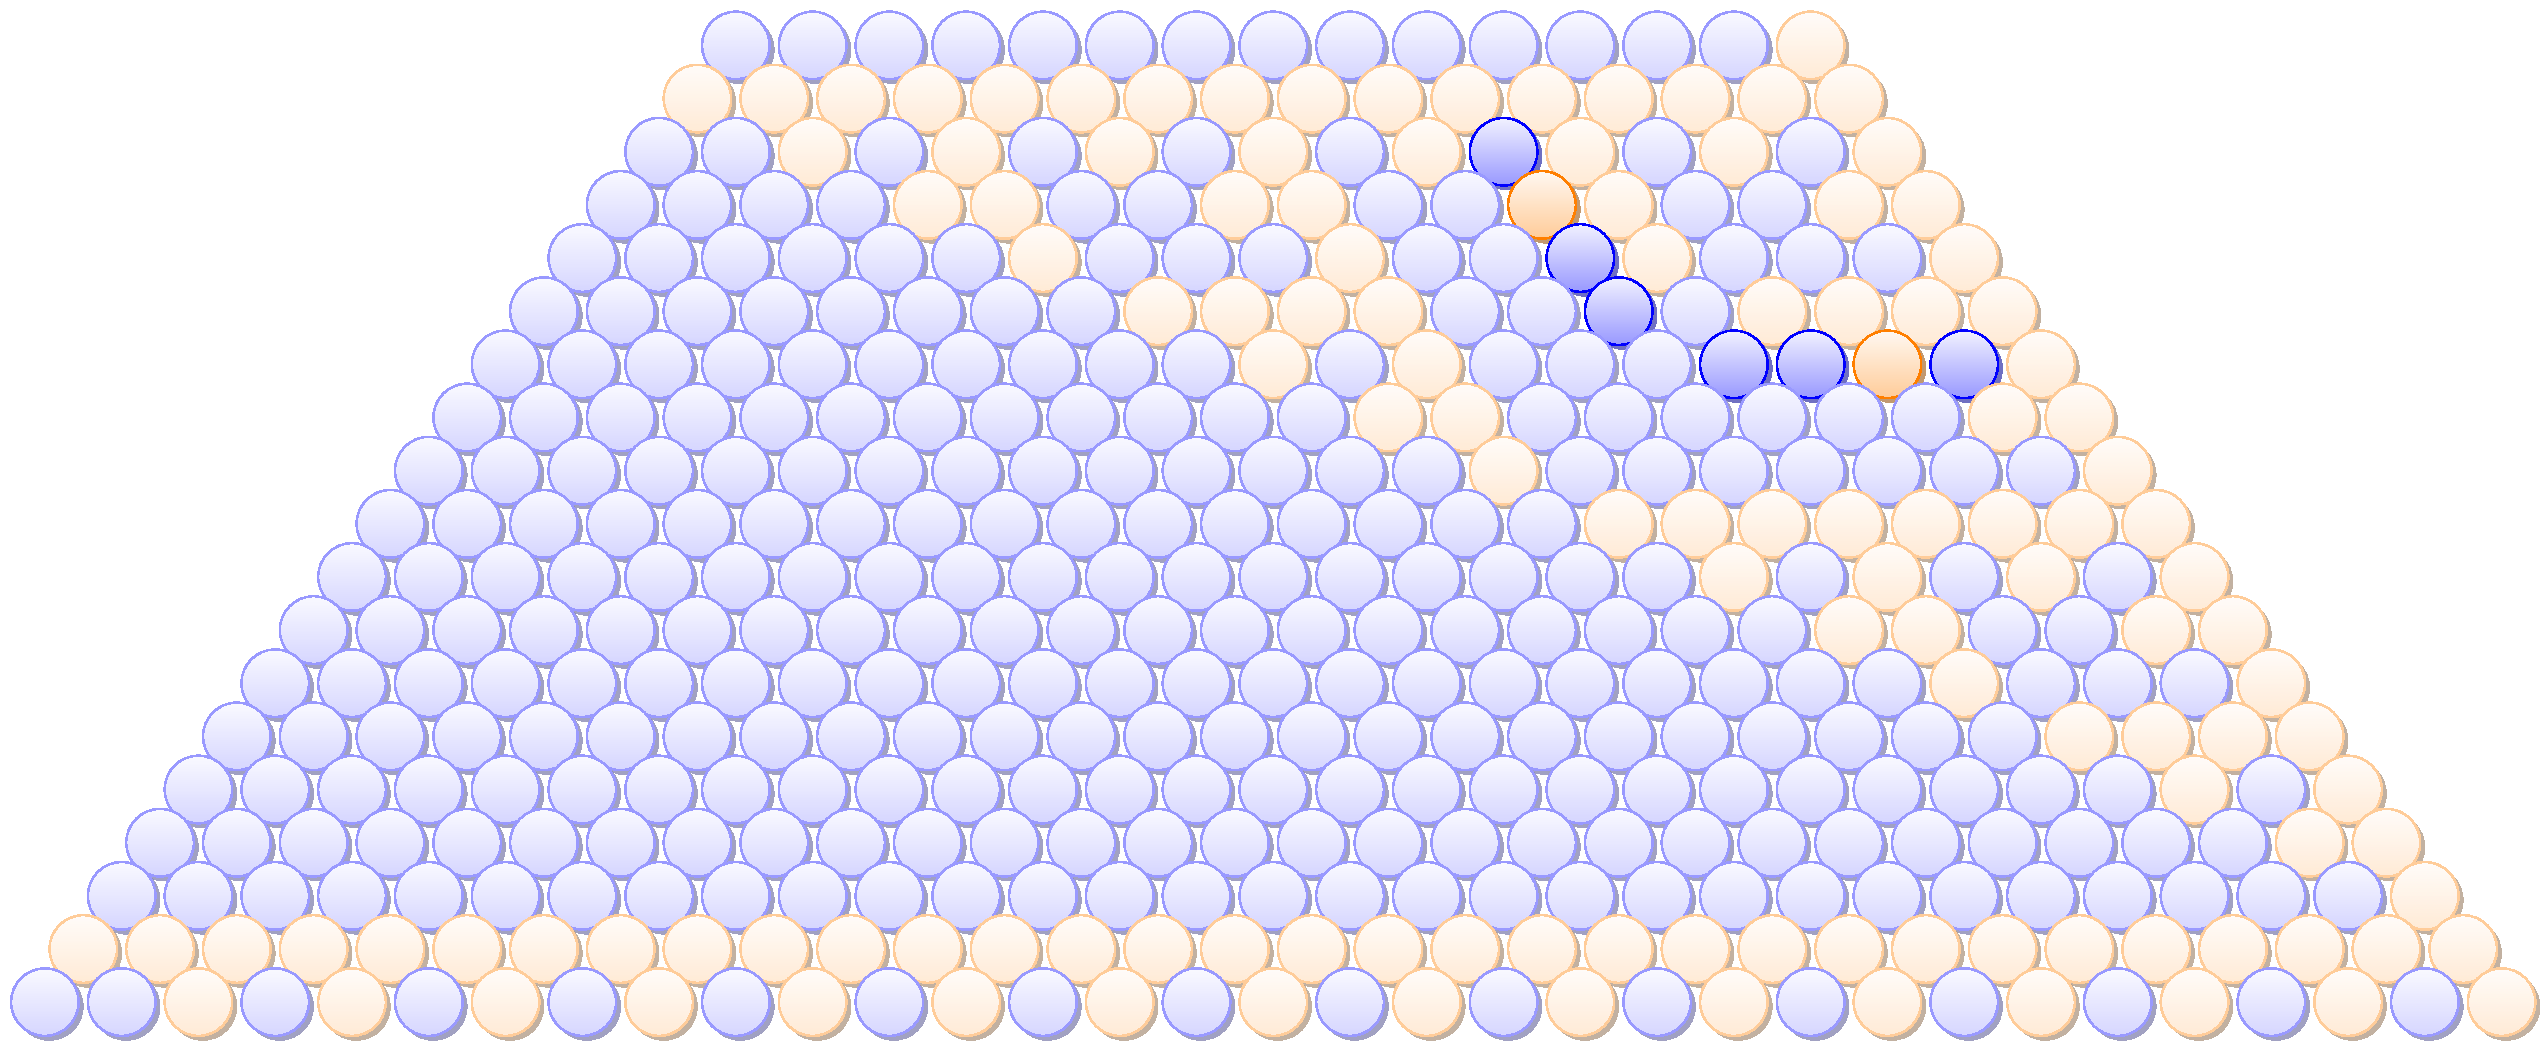
\includegraphics[width=10cm, height=10cm, keepaspectratio=true]
            {../RART2015/catalan-tikz/mirrored-clusters/mirrored-clusters.pdf}
    }

    % this 'particular' line is necessary to use `displaymath' environment
    % into the caption environment, togheter with the inclusion of 
    % `caption' package. See here for more explanation:
    % http://stackoverflow.com/questions/2716227/adding-an-equation-or-formula-to-a-figure-caption-in-latex
    \captionsetup{singlelinecheck=off}
    \caption[\emph{Mirrored} principal clusters $\mathcal{C}_{\equiv_{2}}^{(4)}$]
        {Some coefficients in \emph{mirrored} cluster $\mathcal{C}_{\equiv_{2}}^{(4)}$ 
        over $\hat{d}_{20,2^{4}-1}$: congruences $d_{20-e,2^{4}-1-e} \equiv_{2} d_{20,2^{4}-1+e}$ 
        for $e\in\lbrace1,\ldots,4\rbrace$ }

    \label{fig:catalan-mirrored-clusters}

\end{figure}

In \autoref{fig:catalan-mirrored-clusters} some coefficients in \flqq mirrored\frqq\,
cluster $\mathcal{C}_{\equiv_{2}}^{(4)}$ are highlighted.

\subsection{$\mathcal{C}_{\equiv_{2}}^{(\alpha+1)}$ 
    contains a copy of $\mathcal{C}_{\equiv_{2}}^{(\alpha)}$}

In order to fully characterize $\mathcal{C}$ in a modular context we are
left with a last theorem.

\begin{theorem}

    $\mathcal{C}_{\equiv_{2}}^{(\alpha+1)}$ 
    contains, located at the very right of its bottom strip,
    a copy of $\mathcal{C}_{\equiv_{2}}^{(\alpha)}$.

\end{theorem}

In order to formally state the above question we reason as before, choosing a
\emph{pivot} element lying on the \flqq mirror\frqq\,segment of column
$\vect{c}_{2^{{\alpha}}-1}$. Denote with $S_{2^{{\alpha}}-1}=\lbrace
2^{{\alpha}}+1,\ldots,2^{{\alpha}+1}-2 \rbrace$ the segment of such column and
let coefficient $\hat{d}_{s,2^{{\alpha}}-1}$, where $s\in S_{2^{{\alpha}}-1}$,
be the ``pivot'' element. The request can be formalized as follow:

\begin{displaymath}
    d_{s,2^{{\alpha}}-1+e} \equiv_{2} d_{s-2^{{\alpha}},e-1}
\end{displaymath}
for $e\in\lbrace1,\ldots,s-(2^{{\alpha}}-1)-1\rbrace=\lbrace1,\ldots,s-2^{{\alpha}}\rbrace$,
computed looking at row $s$ toward its end.

\begin{proof}
We tackle the proof using the following definition for $d_{nk}\in\mathcal{C}$:
\begin{displaymath}
    d_{nk}={{2n-k}\choose{n-k}} - {{2n-k}\choose{n-k-1}}
\end{displaymath}
instantiated with our indices, we have to prove:

\begin{lenghtydisplaymath}
    \begin{split}
        {{2s-(2^{{\alpha}}-1+e)}\choose{s-(2^{{\alpha}}-1+e)}} - {{2s-(2^{{\alpha}}-1+e)}\choose{s-(2^{{\alpha}}-1+e)-1}}
        &\equiv_{2}
        {{2(s-2^{{\alpha}})-(e-1)}\choose{(s-2^{{\alpha}})-(e-1)}} - {{2(s-2^{{\alpha}})-(e-1)}\choose{(s-2^{{\alpha}})-(e-1)-1}}\\
        {{2s-2^{{\alpha}}+1-e}\choose{s-2^{{\alpha}}+1-e}} - {{2s-2^{{\alpha}}+1-e}\choose{s-2^{{\alpha}}-e}}
        &\equiv_{2}
        {{2s-2^{{\alpha}+1}-e+1}\choose{s-2^{{\alpha}}-e+1}} - {{2s-2^{{\alpha}+1}-e+1}\choose{s-2^{{\alpha}}-e}}\\
        {{2s-2^{{\alpha}}+1-e}\choose{s}} - {{2s-2^{{\alpha}}+1-e}\choose{s+1}}
        &\equiv_{2}
        {{2s-2^{{\alpha}+1}-e+1}\choose{s-2^{{\alpha}}}} - {{2s-2^{{\alpha}+1}-e+1}\choose{s-2^{{\alpha}}+1}}\\
    \end{split}
\end{lenghtydisplaymath}
Since $e\in\lbrace1,\ldots,s-2^{{\alpha}}\rbrace$, proceed by complete induction on $e$:
    \begin{itemize}
        \item base case $e=1$ therefore:

            \begin{lenghtydisplaymath}
                \begin{split}
                    {{2s-2^{{\alpha}}}\choose{s}} - {{2s-2^{{\alpha}}}\choose{s+1}}
                    &\equiv_{2}
                    {{2s-2^{{\alpha}+1}}\choose{s-2^{{\alpha}}}} - {{2s-2^{{\alpha}+1}}\choose{s-2^{{\alpha}}+1}}\\
                \end{split}
            \end{lenghtydisplaymath}
            In the previous proof a detailed (and boring) derivation has been performed,
            here we observe that upper terms of each binomial coefficient, $2s-2^{{\alpha}}$
            and $2s-2^{{\alpha}+1}$ respectively, have $2$ in their prime factorization, therefore
            expanding each binomial, $2$ can be factored out in turn, making congruent $0$
            each one of them. However an approach similar to the previous one can be
            taken as well.

        \item assume the argument holds for $k\leq e$ and prove for $k=e+1$, so we need to show:

            \begin{lenghtydisplaymath}
                \begin{split}
                    {{2s-2^{{\alpha}}+1-(e+1)}\choose{s}} - {{2s-2^{{\alpha}}+1-(e+1)}\choose{s+1}}
                    &\equiv_{2}
                    {{2s-2^{{\alpha}+1}-(e+1)+1}\choose{s-2^{{\alpha}}}} - {{2s-2^{{\alpha}+1}-(e+1)+1}\choose{s-2^{{\alpha}}+1}}\\
                    {{2s-2^{{\alpha}}-e}\choose{s}} - {{2s-2^{{\alpha}}-e}\choose{s+1}}
                    &\equiv_{2}
                    {{2s-2^{{\alpha}+1}-e}\choose{s-2^{{\alpha}}}} - {{2s-2^{{\alpha}+1}-e}\choose{s-2^{{\alpha}}+1}}\\
                \end{split}
            \end{lenghtydisplaymath}
            which follows directly by complete induction hypothesis.
    \end{itemize}
\end{proof}


\begin{figure}[p]

    \noindent\makebox[\textwidth]{
        \centering
        %\includegraphics[width=0.8\textwidth]{../../sympy/catalan/coloured.pdf}

        % using *angle* property to rotate it is difficult to properly align it
        % in order to have a "real" matrix representation.
        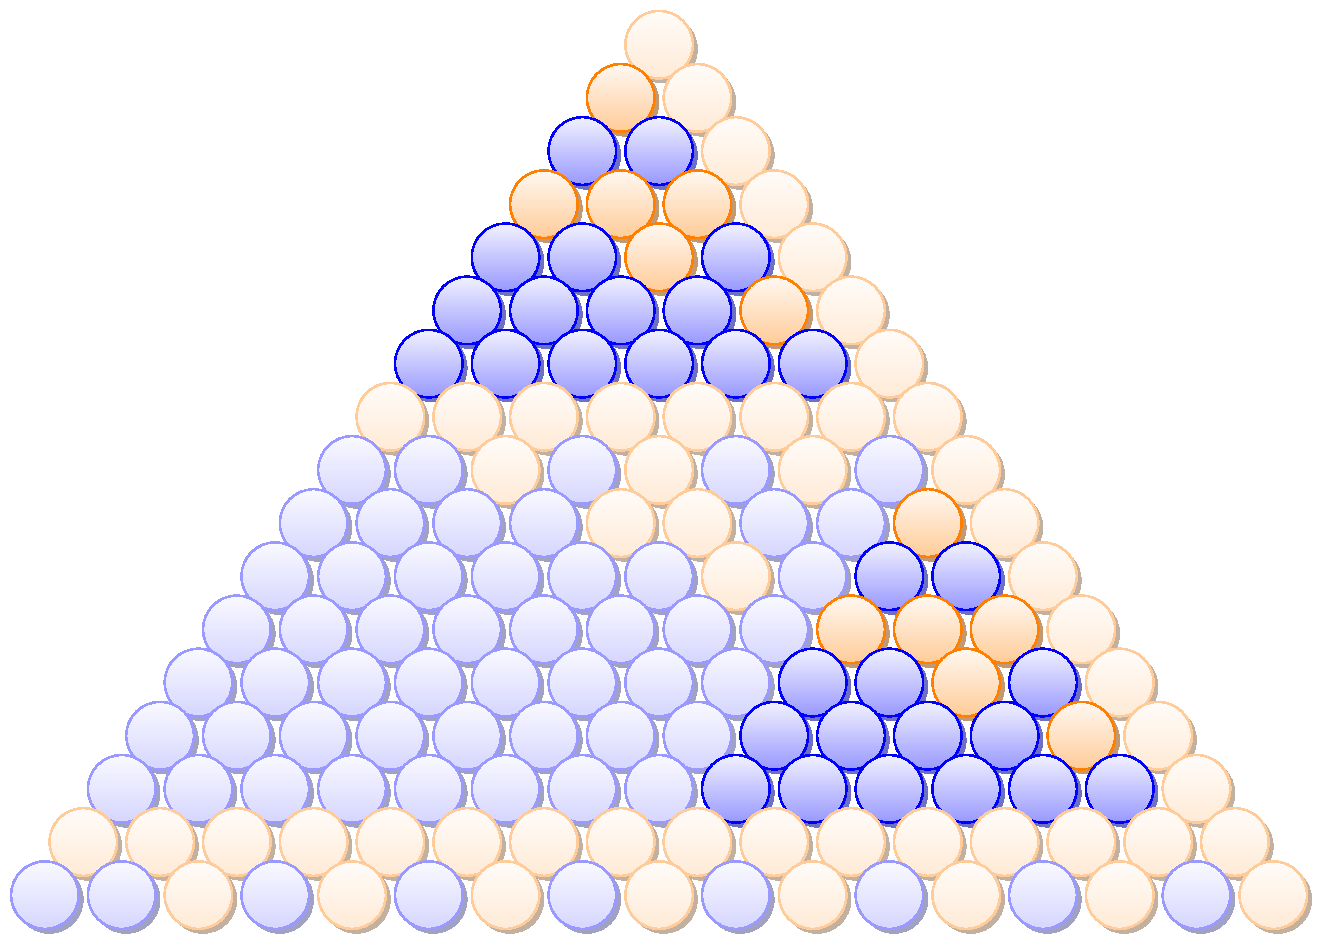
\includegraphics[width=6cm, height=6cm, keepaspectratio=true]{../RART2015/catalan-tikz/principal-cluster/principal-cluster.pdf}
    }

    % this 'particular' line is necessary to use `displaymath' environment
    % into the caption environment, togheter with the inclusion of 
    % `caption' package. See here for more explanation:
    % http://stackoverflow.com/questions/2716227/adding-an-equation-or-formula-to-a-figure-caption-in-latex
    \captionsetup{singlelinecheck=off}
    \caption[$\mathcal{C}_{\equiv_{2}}^{(4)}$ 
    contains a copy of $\mathcal{C}_{\equiv_{2}}^{(3)}$]{$\hat{d}_{s,2^{3}-1}$ for $s\in S_{2^{3}-1}$,
    $d_{s,2^{3}-1+e} \equiv_{2} d_{s-2^{3},e-1}$ with $e\in\lbrace1,\ldots,s-2^{3}\rbrace$ }

    \label{fig:catalan-principal-cluster}

\end{figure}


Before concluding this section, we would like to note that the last two
proofs doesn't say anything about the remainder of a coefficient belonging
to subtriangles of interest: we've shown only that a \emph{complete}
subtriangle is repeated when coefficients are taken modulo $2$. 

Enough for this characterization modulo $2$ for Catalan array $\mathcal{C}$.

\subsection{Some open questions}
% TODO ask how show the modular characterization of the inverse of C, formally

\begin{figure}[p]

    \noindent\makebox[\textwidth]{
        \centering
        %\includegraphics[width=0.8\textwidth]{../../sympy/catalan/coloured.pdf}

        % using *angle* property to rotate it is difficult to properly align it
        % in order to have a "real" matrix representation.
        \includegraphics[width=20cm, height=20cm, keepaspectratio=true]{../sympy/catalan/catalan-traditional-inverse-ignore-negatives-centered-colouring-127-rows-mod2-partitioning-triangle.pdf}
    }

    % this 'particular' line is necessary to use `displaymath' environment
    % into the caption environment, togheter with the inclusion of 
    % `caption' package. See here for more explanation:
    % http://stackoverflow.com/questions/2716227/adding-an-equation-or-formula-to-a-figure-caption-in-latex
    \captionsetup{singlelinecheck=off}
    \caption[$\mathcal{C}_{\equiv_{2}}^{-1}$]{
        Catalan traditional triangle, formally: 
        \begin{displaymath}
            \mathcal{C}^{-1}=\left(t, t {\left(1-t\right)} \right)
        \end{displaymath} % \newline % new line no more necessary
        inverse, ignore negatives, centered colouring, 127 rows, mod2 partitioning
        }

    \label{fig:catalan-traditional-inverse-ignore-negatives-centered-colouring-127-rows-mod2-partitioning-triangle}

\end{figure}

What about a formal proof for the modular characterization of $\mathcal{C}_{\equiv_{2}}^{-1}$, reported in 
\autoref{fig:catalan-traditional-inverse-ignore-negatives-centered-colouring-127-rows-mod2-partitioning-triangle}?

And in general, how generalize to an arbitrary prime $p$?
